\chapter{HASIL DAN PEMBAHASAN}
Pada bab ini dibahas mengenai pengujian dari aplikasi yang telah dikembangkan untuk mengetahui performa aplikasi dalam mendeteksi pose semaphore sesuai tujuan dari penelitian ini, sebagai upaya menciptakan aplikasi yang dapat melakukan prediksi pose semaphore berbasis Deep Learning.

\section{Dataset}
Dalam penelitian ini, dilakukan pengujian terhadap dataset citra yang terdiri dari 26 huruf alfabet yang umum digunakan sehari-hari. Dataset tersebut digunakan untuk melatih dan menguji model dalam mengenali huruf-huruf tersebut. Setiap huruf alfabet direpresentasikan oleh 1000 citra dalam dataset yang digunakan. Pengujian dilakukan untuk mengukur performa dan keakuratan model dalam mengenali huruf-huruf tersebut.

\begin{figure}[!hbt]
	\centering
	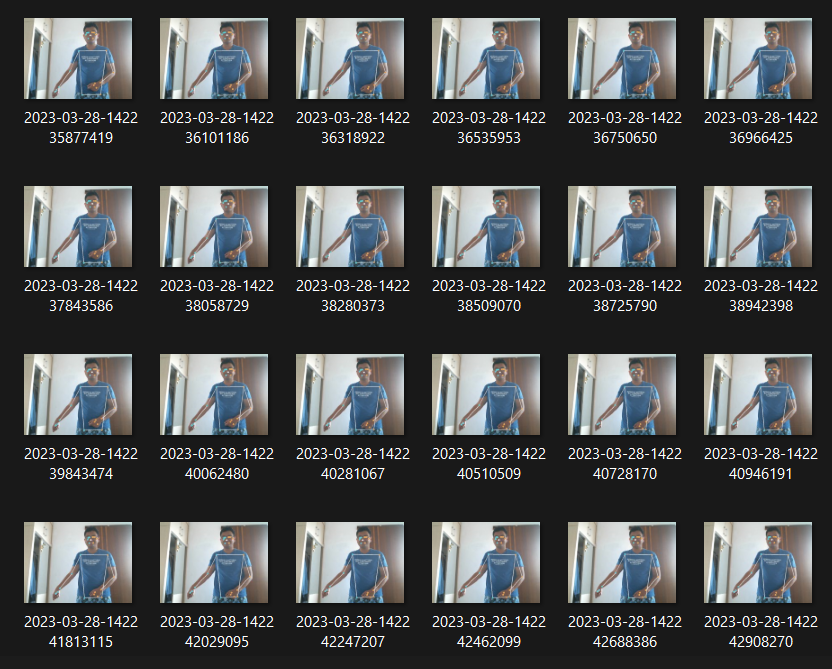
\includegraphics[width=0.7\linewidth]{gambar/citra_dataset.png}
	\captionof{figure}{Dataset Sebelum Ekstraksi}
	\label{fig:Datasetraw}
\end{figure}

Dataset awal yang terdiri dari gambar dan skeleton yang dikombinasikan, yang awalnya diperoleh melalui MediaPipe, akan melalui proses ekstraksi. Proses ekstraksi dilakukan menggunakan program yang telah dikembangkan, menghasilkan skeleton dengan latar belakang hitam. Hasil ekstraksi ini dapat dilihat dalam Gambar \ref{fig:Datasetekstark}.

\begin{figure}[!hbt]
	\centering
	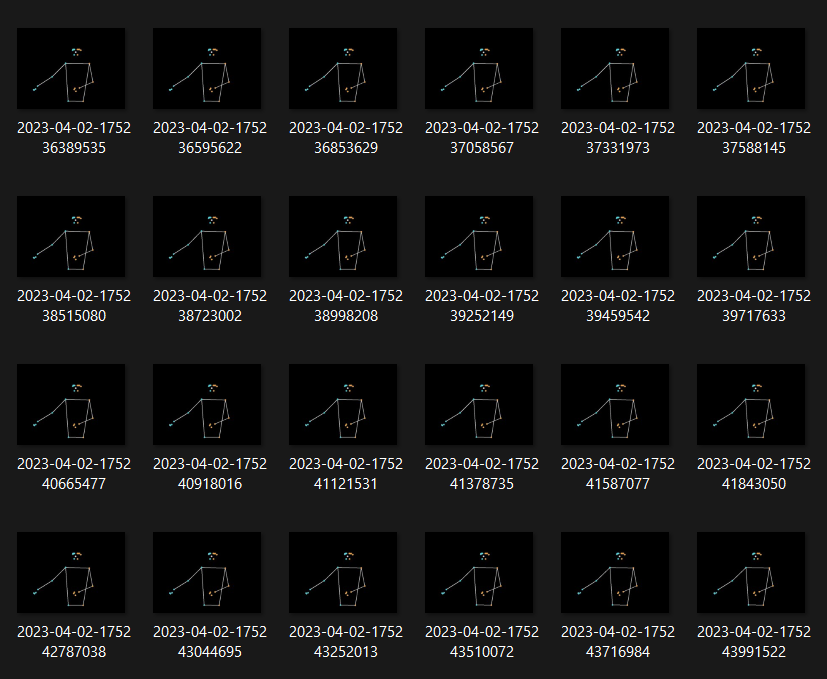
\includegraphics[width=0.7\linewidth]{gambar/tugas-akhir-dawe.png}
	\captionof{figure}{Ekstraksi dari Dataset awal}
	\label{fig:Datasetekstark}
\end{figure}
Dataset yang telah diekstrak ini dijadikan sebagai input dari model-model deep learning pada penelitian ini untuk training dan validasi. 

\begin{table}[htbp]
	\centering
	\captionof{table}{Daftar Dataset}
	\label{tab:datasethuruf}
	\begin{tabular}{|c|c|c|c|c|}
		\hline
		A & B & C & D & E \\
		\hline
		F & G & H & I & J \\
		\hline
		K & L & M & N & O \\
		\hline
		P & Q & R & S & T \\
		\hline
		U & V & W & X & Y \\
		\hline
		Z &   Akhir &   &   &   \\
		\hline
	\end{tabular}
\end{table}

Adapun huruf yang digunakan sebagai dataset bisa dilihat pada tabel \ref{tab:datasethuruf} . Dimana seluruh huruf memiliki bentuk yang statik atau tidak berubah

\section{Model CNN}

Pada awalnya, fungsi ini menerima parameter JumlahKelas yang mengindikasikan jumlah kelas dalam dataset yang digunakan. Kemudian, dilakukan inisialisasi input layer dengan ukuran (128, 128, 3) yang sesuai dengan dimensi gambar pada dataset.

Selanjutnya, dilakukan serangkaian operasi \textit{Conv2D}  dan \textit{MaxPooling2D}. Pertama, terdapat tiga layer \textit{Conv2D} yang masing-masing memiliki 32 \textit{neuron} dengan \textit{filter} berukuran 3x3. Aktivasi \textit{ReLU}  digunakan untuk mengaktifkan \textit{neuron}-\textit{neuron} tersebut. \textit{Padding} 'same' juga diterapkan agar ukuran output tetap sama dengan input. Setelah setiap layer \textit{Conv2D}, dilakukan \textit{MaxPooling2D} dengan ukuran \textit{pooling} 2x2 dan \textit{padding} 'same' untuk melakukan \textit{downsampling} dan mengurangi dimensi data.

Selanjutnya, dilakukan layer \textit{Conv2D} lagi dengan 16 \textit{neuron} dan \textit{filter} berukuran 3x3, diikuti oleh \textit{MaxPooling2D} dengan ukuran \textit{pooling} 2x2 dan \textit{padding} 'same'. Langkah ini bertujuan untuk mengekstraksi fitur-fitur yang lebih kompleks dari data.

Setelah melalui serangkaian operasi \textit{Conv2D} dan \textit{MaxPooling2D}, data kemudian diflatten menjadi vektor satu dimensi menggunakan layer Flatten. Hal ini diperlukan agar data dapat dimasukkan ke dalam layer \textit{Dense} yang merupakan layer \textit{fully connected}.

Selanjutnya, data melewati layer \textit{Dense} dengan 16 \textit{neuron} yang menggunakan aktivasi \textit{ReLU}. Tujuan dari layer ini adalah untuk mempelajari pola-pola yang lebih kompleks dari data yang telah diekstraksi sebelumnya. Untuk mencegah overfitting, dilakukan juga layer Dropout dengan tingkat dropout sebesar 0.2.

Selanjutnya, data melewati layer \textit{Dense} kembali dengan 16 \textit{neuron} dan aktivasi \textit{ReLU}. Layer ini bertujuan untuk memperkuat pembelajaran fitur-fitur yang relevan.

Terakhir, data melewati layer \textit{Dense} dengan jumlah \textit{neuron} sesuai dengan JumlahKelas yang digunakan. Aktivasi \textit{softmax} digunakan untuk mendapatkan probabilitas kelas pada output layer. Model CNN ini kemudian dikompilasi menggunakan \textit{mean squared error} sebagai \textit{loss} function dan optimizer \textit{Adam}. Metrik akurasi juga digunakan untuk mengevaluasi performa model. Pada skenario ini menggunakan 30\textit{ epoch} 

\subsection*{Performa dan Fungsionalitas Model CNN Skenario Pertama}

Grafik akurasi dari Model CNN Pertama dapat dilihat pada Gambar \ref{fig:AkurasiCNN1}. Pertama ini merupakan dasar dari skenario-skenario lain yang digunakan dalam penelitian ini. Pada skenario ini, terdapat 4 layer \textit{Conv2D} yang diikuti oleh Maxpooling, dengan jumlah \textit{neuron} pada masing-masing layer \textit{Conv2D} adalah 32, 32, 32, dan 16. Model CNN ini dilatih selama 30\textit{ epoch}.

Grafik \textit{loss} dari Model CNN Pertama dapat dilihat pada Gambar \ref{fig:lossModelCNN1}. \textit{Loss} function digunakan untuk mengukur sejauh mana prediksi model CNN ini mendekati nilai sebenarnya

Pertama ini menjadi landasan untuk pengembangan dan evaluasi skenario-skenario lain dalam penelitian ini. Dengan menggunakan skenario-skenario yang bervariasi, diharapkan dapat mengeksplorasi berbagai konfigurasi model CNN dan memperoleh hasil yang optimal untuk tugas klasifikasi yang diberikan.

\begin{figure}[!hbt]
	\centering
	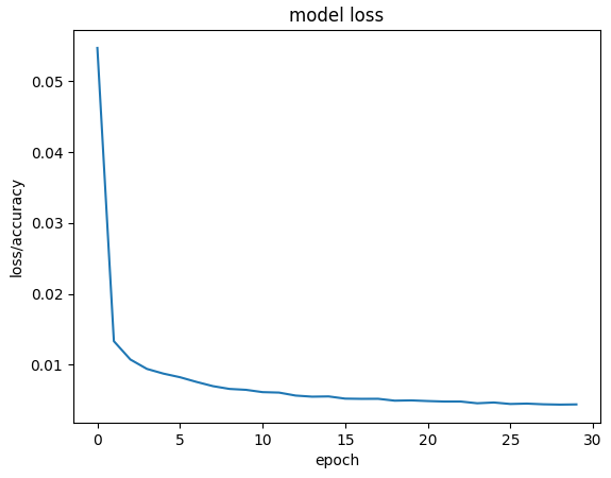
\includegraphics[width=0.7\linewidth]{gambar/bener/Loss_ModelCNN.png}
	\captionof{figure}{Loss Model CNN dengan epoch 30}
	\label{fig:lossModelCNN1}
\end{figure}
Gambar \ref{fig:lossModelCNN1}  menunjukkan perubahan \textit{loss} model selama proses pelatihan 30 siklus (iterasi pelatihan). Kerugian digunakan untuk mengukur seberapa baik prediksi model kita didasarkan pada nilai sebenarnya dari tugas regresi, atau untuk mengukur perbedaan antara prediksi model dan entri yang benar dalam tugas klasifikasi.

Pada awal pelatihan (Epoch 1) \textit{loss} memiliki nilai yang relatif tinggi yaitu sekitar 0,055. Hal ini menunjukkan bahwa model asli masih belum mampu membuat prediksi yang akurat.

Namun seiring dengan kemajuan jaman dan pendidikan, kerugian tersebut berangsur-angsur berkurang dari jaman ke jaman. Semakin kecil nilai kerugian, semakin baik model kita membuat prediksi yang mendekati nilai sebenarnya atau label yang benar.

Di akhir pelatihan (Epoch 30), kerugiannya sekitar 0,0044, menunjukkan bahwa model kami telah berhasil dipelajari dan mampu membuat prediksi yang cukup akurat. 

\begin{figure}[!hbt]
	\centering
	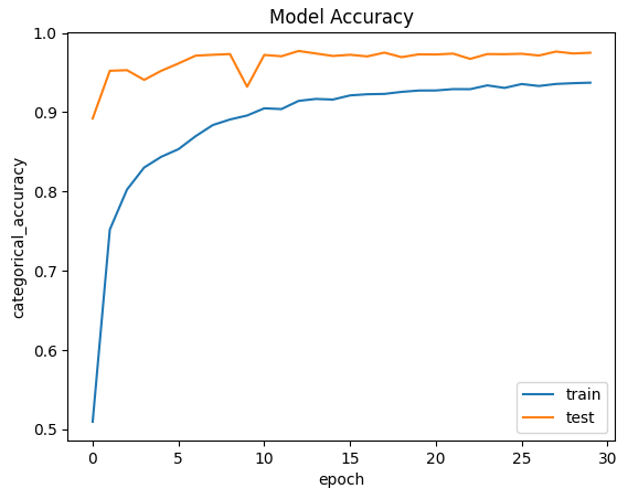
\includegraphics[width=0.7\linewidth]{gambar/bener/Accuracy_ModelCNN.png}
	\captionof{figure}{Akurasi Model CNN dengan epoch 30}
	\label{fig:AkurasiCNN1}
\end{figure}
Gambar \ref{fig:AkurasiCNN1} menunjukkan perubahan akurasi model dan akurasi validasi selama proses pelatihan dalam 30\textit{ epoch}

Pada awal pelatihan (epoch 1), akurasi model relatif rendah, sekitar 50,94\%, sedangkan akurasi validasi cukup tinggi, sekitar 89,20\%. Hal ini menunjukkan bahwa model masih perlu diperbaiki dari segi kemampuan prediksi data pelatihan.

Namun, seiring dengan kemajuan zaman dan kemajuan pendidikan, akurasi model secara bertahap meningkat dari zaman ke zaman. Akurasi konfirmasi juga meningkat dari waktu ke waktu. Pada akhir pelatihan (epoch 30), akurasi model sekitar 93,72\%, sedangkan akurasi validasi sekitar 97,50\%. Grafik ini menunjukkan peningkatan performa model yang berkelanjutan. Keakuratan data pelatihan dan validasi yang ditingkatkan berarti model kami belajar dengan sukses dan dapat menghasilkan prediksi yang lebih akurat dari waktu ke waktu.

Grafik ini menunjukkan peningkatan performa model yang berkelanjutan. Keakuratan data pelatihan dan validasi yang ditingkatkan berarti model kami belajar dengan sukses dan dapat menghasilkan prediksi yang lebih akurat dari waktu ke waktu.  

\begin{figure}[!hbt]
	\centering
	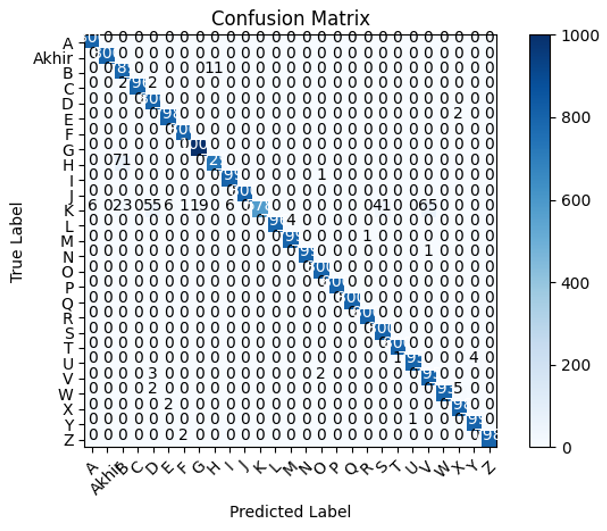
\includegraphics[width=0.7\linewidth]{gambar/bener/ConfusionMatrix_ModelCNN.png}
	\captionof{table}{Tabel Confusion Matriks Model CNN dengan epoch 30}
	\label{fig:TabelModelCNN1}
\end{figure}
Dalam kasus ini, matriks tersebut mencerminkan hasil dari deteksi huruf dalam suatu dataset. Terdapat 26 label huruf, yaitu A sampai Z. Diagonal utama dari matriks menunjukkan jumlah contoh yang diklasifikasikan dengan benar, di mana nilai-nilai tersebut merupakan \textit{True Positives } atau contoh yang benar-benar terdeteksi dengan benar untuk setiap huruf.

Berdasarkan Gambar \ref{fig:TabelModelCNN1}, ditemukan bahwa akurasi deteksi dan label huruf K sebesar 578. Hal ini disebabkan oleh kesalahan dalam dataset label huruf K yang terdapat 185 data pelatihan yang seharusnya berisi huruf V. Kesalahan ini terjadi karena kesalahan dalam pengelompokan data ke dalam folder yang menyebabkan kesalahan dalam mengidentifikasi huruf K sebagai huruf V. Dalam deteksi tersebut, terdapat 65 kasus di mana huruf K salah terdeteksi sebagai huruf V, 19 kasus sebagai huruf G, 23 kasus sebagai huruf B, dan 61 kasus sebagai huruf S.

Beberapa nilai di luar diagonal utama juga menunjukkan adanya kesalahan prediksi. Sebagai contoh, pada baris B dan kolom H terdapat 11 contoh yang seharusnya huruf B tetapi salah terklasifikasi sebagai huruf H \textit{False Positives}. Hal yang sama berlaku untuk kesalahan prediksi lainnya.

Berikut merupakan tabel perhitungan \textit{F1-score}, presisi, dan recall yang dapat dilihat pada Tabel \ref{tbl:TabelModelCNN} menggunakan \textit{Confusion Matrix} pada Gambar \ref{fig:TabelModelCNN1}

\begin{table}[!hbt]
	\centering
	\captionof{table}{Tabel Model CNN Confusion Matrix}
	\label{tbl:TabelModelCNN}
	\begin{tabular}{|c|c|c|c|c|}
	\hline
	Class & Precision & Recall & F1-score & Accuracy \\
	\hline
	A & 0.9926 & 1.0000 & 0.9963 & 1.0000 \\
	Akhir & 1.0000 & 1.0000 & 1.0000 & 1.0000 \\
	B & 0.8915 & 0.9863 & 0.9365 & 0.9863 \\
	C & 1.0000 & 0.9950 & 0.9975 & 0.9950 \\
	D & 0.9281 & 1.0000 & 0.9627 & 1.0000 \\
	E & 0.9901 & 0.9975 & 0.9938 & 0.9975 \\
	F & 0.9963 & 1.0000 & 0.9981 & 1.0000 \\
	G & 0.9814 & 1.0000 & 0.9906 & 1.0000 \\
	H & 0.9851 & 0.9113 & 0.9468 & 0.9113 \\
	I & 0.9925 & 0.9988 & 0.9956 & 0.9988 \\
	J & 1.0000 & 1.0000 & 1.0000 & 1.0000 \\
	K & 1.0000 & 0.7225 & 0.8389 & 0.7225 \\
	L & 1.0000 & 0.9950 & 0.9975 & 0.9950 \\
	M & 0.9950 & 0.9988 & 0.9969 & 0.9988 \\
	N & 1.0000 & 0.9988 & 0.9994 & 0.9988 \\
	O & 0.9963 & 1.0000 & 0.9981 & 1.0000 \\
	P & 1.0000 & 1.0000 & 1.0000 & 1.0000 \\
	Q & 1.0000 & 1.0000 & 1.0000 & 1.0000 \\
	R & 0.9988 & 1.0000 & 0.9994 & 1.0000 \\
	S & 0.9513 & 1.0000 & 0.9750 & 1.0000 \\
	T & 0.9988 & 1.0000 & 0.9994 & 1.0000 \\
	U & 0.9987 & 0.9938 & 0.9962 & 0.9938 \\
	V & 0.9233 & 0.9938 & 0.9573 & 0.9938 \\
	W & 1.0000 & 0.9913 & 0.9956 & 0.9913 \\
	X & 0.9913 & 0.9975 & 0.9944 & 0.9975 \\
	Y & 0.9950 & 0.9988 & 0.9969 & 0.9988 \\
	Z & 1.0000 & 0.9975 & 0.9987 & 0.9975 \\
	\hline
	\end{tabular}
\end{table}

Untuk rata-rata metrik evaluasi, Accuracy mencapai 98.94\%, Recall mencapai 99.75\%, \textit{Precision} mencapai 98.62\%, dan \textit{F1-score} mencapai 99.13\%. Hal ini menunjukkan bahwa secara keseluruhan, model CNN memiliki performa yang sangat baik dalam mengklasifikasikan huruf-huruf dalam dataset.


\section{Model CNN Kedua}
Pada Model CNN Kedua , Dataset tersebut melewati beberapa lapisan untuk mengekstraksi fitur. Pertama, dataset melewati lapisan \textit{Conv2D} dengan 32 \textit{neuron}, \textit{filter} 3x3, aktivasi \textit{ReLU}, dan \textit{padding} yang sama. Kemudian, dilakukan \textit{MaxPooling2D} dengan ukuran \textit{pooling} 2x2 dan \textit{padding} yang sama.

Selanjutnya, dataset melewati lapisan \textit{Conv2D} lain dengan 16 \textit{neuron}, \textit{filter} 3x3, aktivasi \textit{ReLU}, dan \textit{padding} yang sama sebanyak dua kali. Kemudian dilakukan lagi \textit{MaxPooling2D} dengan ukuran \textit{pooling} 2x2 dan \textit{padding} yang sama. Dan diakhiri dengan dataset melewati lapisan \textit{Conv2D} dengan 8 \textit{neuron} , \textit{filter} 3x3 , aktivasi \textit{ReLU} dan \textit{padding} yang sama sebanyak dua kali serta \textit{MaxPooling2D} dengan ukuran \textit{pooling} 2x2 

Setelah proses ekstraksi fitur, dataset kemudian masuk ke tahap klasifikasi. Pertama, dilakukan flattening untuk mengubah data menjadi vektor satu dimensi. Kemudian, data melewati lapisan \textit{Dense} dengan 16 \textit{neuron} dan aktivasi \textit{ReLU}. Untuk mencegah overfitting, dilakukan dropout dengan dropout rate 0.2. Setelah itu, terdapat lapisan \textit{Dense} lagi dengan 16 \textit{neuron} dan aktivasi \textit{ReLU}. Lapisan terakhir menggunakan \textit{Dense} dengan jumlah \textit{neuron} sesuai dengan jumlah kelas pada dataset (JumlahKelas) dan aktivasi \textit{softmax} untuk menghasilkan output probabilitas kelas. Model CNN ini menggunakan fungsi \textit{loss} \textit{mean squared error} dan optimizer \textit{Adam} dalam proses kompilasi

Grafik akurasi dari Model CNN Kedua tersedia di Gambar \ref{fig:AkurasiCNNKedua}. Dalam skenario ini, terdapat empat lapisan \textit{Conv2D} yang diikuti oleh \textit{Maxpooling}. Jumlah \textit{neuron} dalam setiap lapisan \textit{Conv2D} adalah 32, 16, 16, dan 8. Model CNN ini dilatih selama 30\textit{ epoch}.

Grafik \textit{loss} dari Model CNN Kedua dapat ditemukan di Gambar \ref{fig:lossModelCNNKedua}. \textit{Loss} function digunakan untuk mengukur sejauh mana prediksi model CNN mendekati nilai sebenarnya. Pada skenario ini, model CNN berhasil mengurangi \textit{loss} secara signifikan selama proses pelatihan selama 30\textit{ epoch}.

\begin{figure}[!hbt]
	\centering
	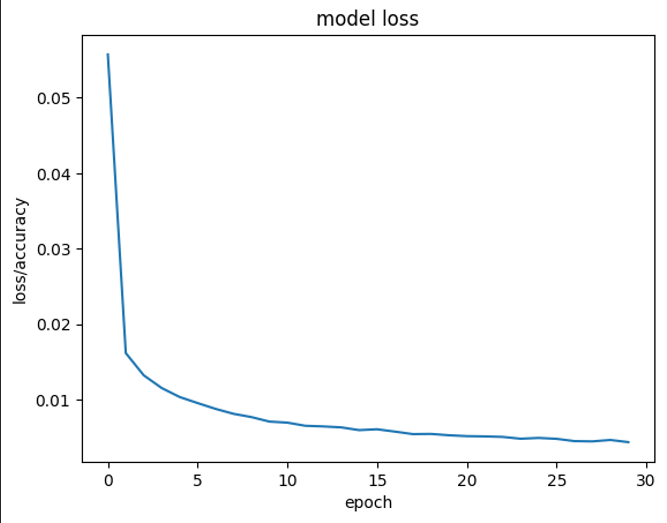
\includegraphics[width=0.7\linewidth]{gambar/bener/Loss_ModelCNN2.png}
	\captionof{figure}{Loss Model CNN 2 dengan epoch 30}
	\label{fig:lossModelCNNKedua}
\end{figure}

Seperti terlihat pada \ref{fig:lossModelCNNKedua}, \textit{loss} pada awal pelatihan (epoch 1) memiliki nilai yang relatif tinggi yaitu sekitar 0,056. Hal ini menunjukkan bahwa model asli masih belum mampu membuat prediksi yang akurat.

Namun seiring dengan kemajuan jaman dan pendidikan, kerugian tersebut berangsur-angsur berkurang dari jaman ke jaman. Semakin kecil nilai kerugian, semakin baik model kita membuat prediksi yang mendekati nilai sebenarnya atau label yang benar.

Di akhir pelatihan (epoch 30), \textit{loss} sekitar 0,00434, menunjukkan bahwa model kita telah berhasil dipelajari dan mampu membuat prediksi yang cukup akurat. Grafik ini menunjukkan proses pelatihan yang sukses, dengan kerugian terus menerus dan terus menurun dari musim ke musim. Ini menunjukkan bahwa model kami secara bertahap menangkap pola-pola penting dalam data dan meningkatkan prediktabilitas. 

\begin{figure}[!hbt]
	\centering
	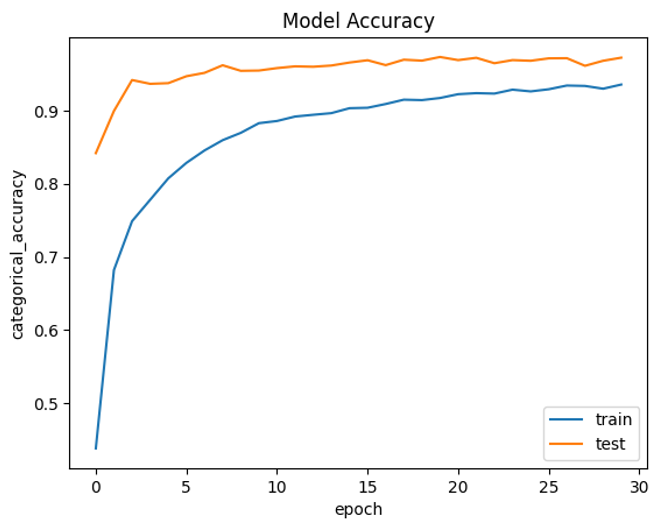
\includegraphics[width=0.7\linewidth]{gambar/bener/Accuracy_ModelCNN2.png}
	\captionof{figure}{Akurasi Model CNN 2 dengan epoch 30}
	\label{fig:AkurasiCNNKedua}
\end{figure}

Seperti terlihat pada Gambar \ref{fig:AkurasiCNNKedua}, akurasi model pada awal pelatihan (epoch 1) relatif rendah sekitar 43,85\%, sedangkan akurasi validasi cukup tinggi sekitar 84,17\%. Hal ini menunjukkan bahwa model asli masih perlu diperbaiki dalam hal kemampuan prediksi data pelatihan.

Namun, seiring dengan berjalannya\textit{ epoch} dan pelatihan, Akurasi model secara bertahap meningkat dari zaman ke zaman. Akurasi konfirmasi juga meningkat dari waktu ke waktu. Pada akhir pelatihan (epoch 30), akurasi model sekitar 93,53\%, sedangkan akurasi validasi sekitar 97,20\%. Gambar 10 menunjukkan peningkatan berkelanjutan dalam kinerja model. Keakuratan data pelatihan dan validasi yang lebih baik berarti bahwa model kami belajar dengan sukses dan dapat membuat prediksi yang lebih akurat dari waktu ke waktu. 	

\begin{figure}[!hbt]
	\centering
	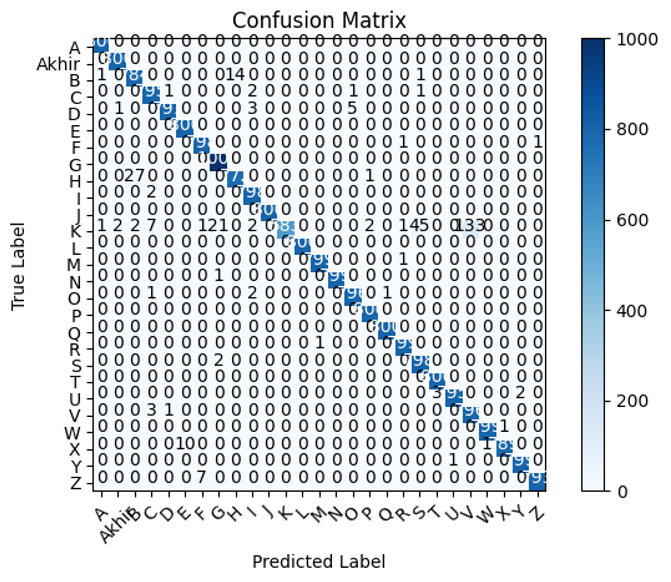
\includegraphics[width=0.7\linewidth]{gambar/bener/ConfusionMatrix_ModelCNN2.png}
	\captionof{table}{Tabel Confusion Matriks Model CNN Kedua dengan epoch 30}
	\label{fig:TabelModelCNNKedua}
\end{figure}
Berdasarkan Gambar \ref{fig:lossModelCNNKedua}, dapat dilihat bahwa dalam kasus deteksi dan label huruf K, terdapat akurasi sebesar 583. Hal ini disebabkan oleh adanya kesalahan dalam memasukkan dataset ke dalam folder training, sehingga dataset label huruf K sebenarnya juga mencakup huruf V. Sebagai akibatnya, model mengalami kesulitan dalam membedakan antara huruf K dan huruf V saat melakukan deteksi.

Dalam kasus ini, terdapat beberapa kesalahan deteksi yang menyebabkan nilai-nilai dalam \textit{Confusion Matrix} menjadi signifikan. Sebagai contoh, terdapat 7 kasus di mana huruf K salah terdeteksi sebagai huruf C, 21 kasus sebagai huruf G, 2 kasus sebagai huruf B, 2 kasus sebagai kata "Akhir", 45 kasus sebagai huruf S, dan 133 kasus sebagai huruf V. Kesalahan ini terjadi karena perbedaan bentuk dan fitur antara huruf K dan huruf V yang mungkin sulit untuk dikenali oleh model.

Berikut merupakan tabel perhitungan \textit{F1-score}, presisi, dan recall yang dapat dilihat pada Tabel \ref{tbl:ModelCNN2CONFUSIONMATRIX} menggunakan \textit{Confusion Matrix} pada Gambar \ref{fig:TabelModelCNNKedua}

\begin{center}
	\begin{table}[!hbt]
	\centering
	\captionof{table}{Tabel Model CNN 2 Confusion Matrix}
	\label{tbl:ModelCNN2CONFUSIONMATRIX}
	\begin{tabular}{|c|c|c|c|c|}
	\hline
	Class & Precision & Recall & F1-score & Accuracy \\
	\hline
	A & 0.9975 & 1.0000 & 0.9988 & 1.0000 \\
	Akhir & 0.9963 & 1.0000 & 0.9981 & 1.0000 \\
	B & 0.9643 & 0.9800 & 0.9721 & 0.9800 \\
	C & 0.9839 & 0.9938 & 0.9888 & 0.9938 \\
	D & 0.9975 & 0.9888 & 0.9931 & 0.9888 \\
	E & 0.9877 & 1.0000 & 0.9938 & 1.0000 \\
	F & 0.9901 & 0.9975 & 0.9938 & 0.9975 \\
	G & 0.9766 & 1.0000 & 0.9881 & 1.0000 \\
	H & 0.9822 & 0.9650 & 0.9735 & 0.9650 \\
	I & 0.9888 & 0.9975 & 0.9932 & 0.9975 \\
	J & 1.0000 & 1.0000 & 1.0000 & 1.0000 \\
	K & 1.0000 & 0.7288 & 0.8431 & 0.7288 \\
	L & 1.0000 & 1.0000 & 1.0000 & 1.0000 \\
	M & 0.9988 & 0.9988 & 0.9988 & 0.9988 \\
	N & 1.0000 & 0.9988 & 0.9994 & 0.9988 \\
	O & 0.9925 & 0.9950 & 0.9938 & 0.9950 \\
	P & 0.9963 & 1.0000 & 0.9981 & 1.0000 \\
	Q & 0.9988 & 1.0000 & 0.9994 & 1.0000 \\
	R & 0.9963 & 0.9988 & 0.9975 & 0.9988 \\
	S & 0.9444 & 0.9975 & 0.9702 & 0.9975 \\
	T & 0.9963 & 1.0000 & 0.9981 & 1.0000 \\
	U & 0.9987 & 0.9938 & 0.9962 & 0.9938 \\
	V & 0.8568 & 0.9950 & 0.9208 & 0.9950 \\
	W & 0.9988 & 0.9988 & 0.9988 & 0.9988 \\
	X & 0.9987 & 0.9863 & 0.9925 & 0.9863 \\
	Y & 0.9975 & 0.9988 & 0.9981 & 0.9988 \\
	Z & 0.9987 & 0.9913 & 0.9950 & 0.9913 \\
	\hline
	\end{tabular}
	\end{table}
\end{center}

Berdasarkan Tabel \ref{tbl:ModelCNN2CONFUSIONMATRIX}, model ini mencapai kinerja yang sangat memuaskan dalam mengklasifikasikan kelas yang berbeda. Model tersebut dapat mengidentifikasi berbagai kategori material dengan sangat tepat dengan akurasi 99,1\%. Skor F1 sebesar 99,3\% menunjukkan kemampuan model untuk memperhitungkan positif palsu dan negatif palsu. Tingkat pemulihan sebesar 99,8\% menunjukkan bahwa model tersebut memiliki tingkat keberhasilan yang tinggi dalam mengidentifikasi anggota yang positif. Selain itu, akurasi 98,9\% menunjukkan bahwa model mampu mengklasifikasikan elemen positif dari semua elemen positif dengan benar. 


\section{Model CNN ResNet50v2}
Pada Model CNN ResNet50v2, digunakan arsitektur \textit{ResNet50V2 }sebagai model dasar. \textit{ResNet50V2 }merupakan salah satu arsitektur jaringan saraf konvolusi yang terbukti efektif dalam pengenalan gambar.

\textit{ResNet50V2 }memiliki struktur yang dalam dengan total 50 lapisan. Arsitektur ini menggunakan blok residual untuk mengatasi masalah penurunan performa yang umum terjadi pada jaringan saraf konvolusi yang sangat dalam. Blok residual memanfaatkan koneksi lompatan (skip connection) untuk memperbaiki propagasi gradien, sehingga mengurangi penurunan performa saat jaringan semakin dalam . 

Selanjutnya , hasil keluaran dari model diambil dan diproses menggunakan operasi Global Average \textit{pooling} 2D untuk menghasilkan vektor fitur global dari seluruh gambar . Vektor fitur tersebut kemudian melewati lapisan \textit{Dense} dengan 16 \textit{neuron} dan aktivasi \textit{ReLU}. Untuk menghindari overfitting, dilakukan dropout dengan tingkat dropout sebesar 0.2. Kemudian, terdapat lapisan \textit{Dense} lain dengan 16 \textit{neuron} dan aktivasi \textit{ReLU}. Lapisan terakhir menggunakan \textit{Dense} dengan jumlah \textit{neuron} sesuai dengan jumlah kelas pada dataset (JumlahKelas) dan aktivasi \textit{softmax} untuk menghasilkan probabilitas kelas sebagai output . 

\subsection*{Performa dan Fungsionalitas Model CNN \textit{ResNet50v2 }Skenario Pertama}

Grafik akurasi dari Model CNN \textit{ResNet50V2 }tersedia pada Gambar \ref{fig:AkurasiCNNResNet50V2}. Pada skenario ini, model CNN menggunakan arsitektur \textit{ResNet50V2 }sebagai base model. Model CNN ini dilatih selama 30\textit{ epoch}.

Grafik \textit{loss} dari Model CNN \textit{ResNet50V2 }dapat dilihat pada Gambar \ref{fig:lossModelCNNResNet50v2}. \textit{Loss} function digunakan untuk mengukur sejauh mana prediksi model mendekati nilai sebenarnya. Pada skenario ini, model CNN berhasil mengurangi \textit{loss} secara signifikan selama proses pelatihan selama 30\textit{ epoch}.

\begin{figure}[!hbt]
	\centering
	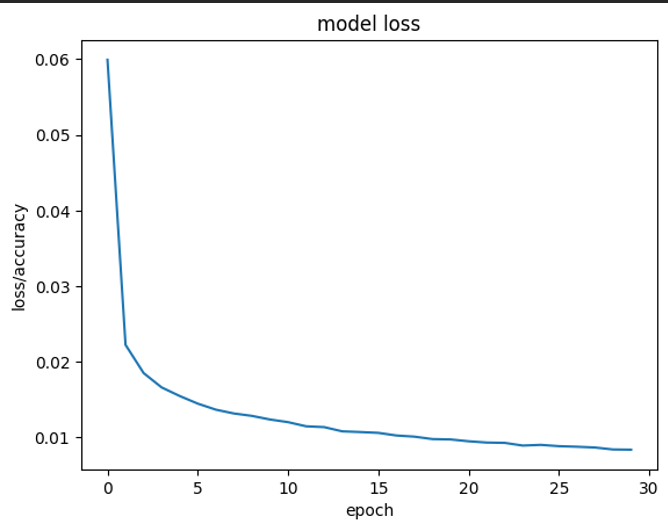
\includegraphics[width=0.7\linewidth]{gambar/bener/Loss_ModelCNNResNet50V2.png}
	\captionof{figure}{Loss Model CNN ResNet50V2 dengan epoch 30}
	\label{fig:lossModelCNNResNet50v2}
\end{figure}

Menurut Gambar\ref{fig:lossModelCNNResNet50v2}, kerugian awal pada awal pelatihan (epoch 1) cukup tinggi, sekitar 0,0599. Namun, seiring bertambahnya jumlah\textit{ epoch}, kerugian secara bertahap berkurang. Hal ini menunjukkan bahwa model secara perlahan mengoptimalkan parameternya untuk meminimalkan perbedaan antara keluaran yang diprediksi dan keluaran aktual.

Dengan setiap\textit{ epoch}, kerugian berkurang, menunjukkan bahwa model lebih baik dalam mempelajari pola dalam data pelatihan. Di musim terakhir (Epoch 30), kerugian berkurang menjadi sekitar 0,0084, menunjukkan bahwa model mencapai akurasi yang baik dalam memprediksi kelas yang benar. Pengurangan kerugian ini menunjukkan bahwa model CNN \textit{Xception} berhasil menghasilkan representasi fitur yang kuat dan mempelajari hubungan kompleks antara input gambar dan output kelas. Dengan kata lain, model ini mengenali pola pada gambar dan mengklasifikasikannya dengan akurasi tinggi.  
\begin{figure}[!hbt]
	\centering
	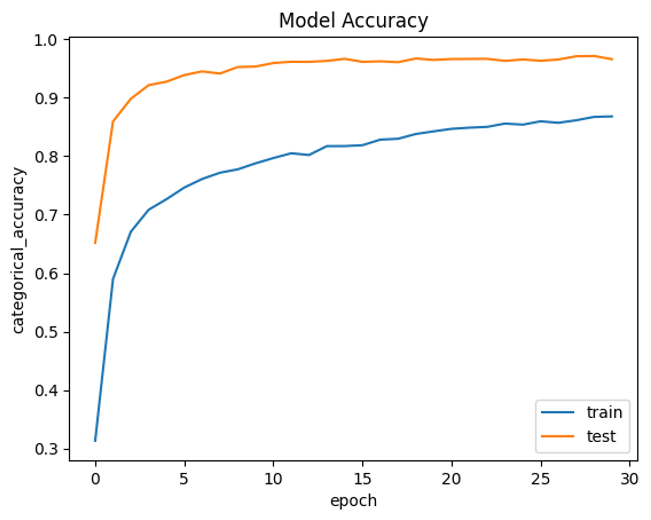
\includegraphics[width=0.7\linewidth]{gambar/bener/Accuracy_ModelResNet50V2.png}
	\captionof{figure}{Akurasi Model CNN ResNet50V2 dengan epoch 30}
	\label{fig:AkurasiCNNResNet50V2}
\end{figure}
Berdasarkan Gambar \ref{fig:AkurasiCNNResNet50V2}, pada awal pelatihan (epoch 1), tingkat akurasi awal rendah, sekitar 0,3134, dan tingkat akurasi validasi sekitar 0,6519. Namun, seiring bertambahnya jumlah\textit{ epoch}, keakuratan data pelatihan dan data validasi secara bertahap meningkat.

Akurasi meningkat pada setiap\textit{ epoch}, menunjukkan bahwa model semakin mampu mempelajari pola dari data pelatihan dan mentransfernya dengan baik ke data validasi. Pada\textit{ epoch} sebelumnya (epoch 30), akurasinya sekitar 86,8\% untuk data training dan 96,59\% untuk data validasi. Hal ini menunjukkan bahwa model mampu mengklasifikasikan citra dengan akurasi yang tinggi.  

\begin{figure}[!hbt]
	\centering
	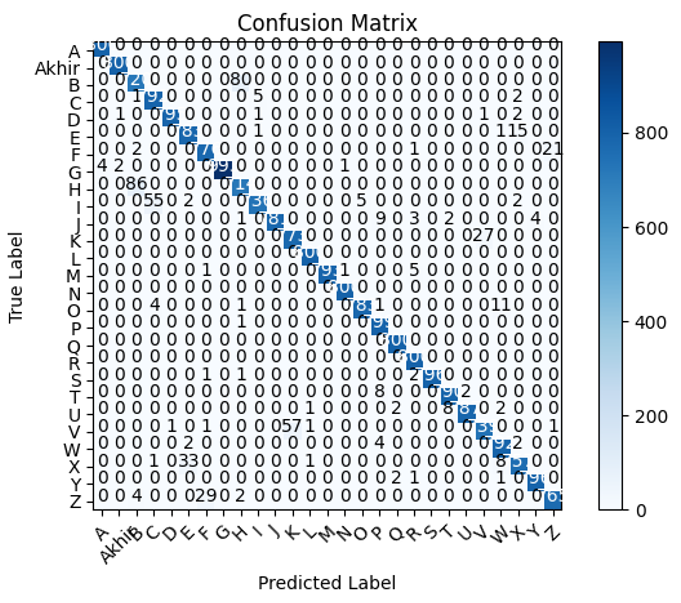
\includegraphics[width=0.7\linewidth]{gambar/bener/ConfusionMatrix_ModelCNNResNet50V2.png}
	\captionof{table}{Tabel Confusion Matriks Model CNN ResNet50V2 dengan epoch 30}
	\label{fig:TabelModelCNNResNet50v2}
\end{figure}
Dalam Tabel \textit{Confusion Matrix} sesuai \ref{fig:TabelModelCNNResNet50v2}, terdapat beberapa hasil yang perlu diperhatikan. Beberapa kelas huruf memiliki nilai \textit{True Poqsitives } yang tinggi, di mana huruf-huruf tersebut diklasifikasikan dengan benar oleh model. Contohnya, huruf A, Akhir, D, E, F, dan G memiliki \textit{True Positives} yang mendekati atau sama dengan 800, menunjukkan bahwa model berhasil mengklasifikasikan huruf-huruf tersebut dengan benar.

Namun, terdapat beberapa kesalahan dalam prediksi model. Sebagai contoh, pada baris B dan kolom H, terdapat 80 contoh yang seharusnya adalah huruf B tetapi salah terklasifikasi sebagai huruf H \textit{False Negatives} . Hal yang sama berlaku untuk kesalahan prediksi pada beberapa kelas huruf lainnya seperti C, I, J, S, U, dan V.

Beberapa nilai di luar diagonal utama juga menunjukkan adanya kesalahan prediksi. Misalnya, pada baris B dan kolom C terdapat 1 contoh yang seharusnya huruf B tetapi salah terklasifikasi sebagai huruf C \textit{False Positives}. Hal yang sama berlaku untuk kesalahan prediksi pada beberapa kelas huruf lainnya.

Matriks juga menunjukkan bahwa beberapa kelas huruf menghadapi kesulitan dalam pengklasifikasian. Sebagai contoh, pada baris K dan kolom K, terdapat 773 contoh yang berhasil diklasifikasikan dengan benar sebagai huruf K (True Positives), tetapi juga terdapat beberapa kesalahan dalam pengklasifikasian, seperti 27 contoh yang salah terklasifikasi sebagai huruf V \textit{False Positives}.

Berikut merupakan tabel perhitungan \textit{F1-score}, presisi, dan recall yang dapat dilihat pada Tabel \ref{tbl:Tabel Confusion Matrix ResNet50V2} menggunakan \textit{Confusion Matrix} pada Gambar \ref{fig:TabelModelCNNResNet50v2}

\begin{table}[!hbt]
	\centering
	\captionof{table}{Tabel Confusion Matrix ResNet50V2}
	\label{tbl:Tabel Confusion Matrix ResNet50V2}
	\begin{tabular}{|c|c|c|c|c|}
	\hline
	Class & Precision & Recall & F1-score & Accuracy \\
	\hline
	A & 0.9950 & 1.0000 & 0.9975 & 1.0000 \\
	Akhir & 0.9963 & 1.0000 & 0.9981 & 1.0000 \\
	B & 0.8856 & 0.9000 & 0.8927 & 0.9000 \\
	C & 0.9296 & 0.9900 & 0.9588 & 0.9900 \\
	D & 0.9987 & 0.9938 & 0.9962 & 0.9938 \\
	E & 0.9549 & 0.9788 & 0.9667 & 0.9788 \\
	F & 0.9604 & 0.9700 & 0.9652 & 0.9700 \\
	G & 1.0000 & 0.9930 & 0.9965 & 0.9930 \\
	H & 0.8925 & 0.8925 & 0.8925 & 0.8925 \\
	I & 0.9906 & 0.9200 & 0.9540 & 0.9200 \\
	J & 1.0000 & 0.9762 & 0.9880 & 0.9762 \\
	K & 0.9313 & 0.9662 & 0.9485 & 0.9662 \\
	L & 0.9963 & 1.0000 & 0.9981 & 1.0000 \\
	M & 1.0000 & 0.9912 & 0.9956 & 0.9912 \\
	N & 0.9975 & 1.0000 & 0.9988 & 1.0000 \\
	O & 0.9937 & 0.9788 & 0.9861 & 0.9788 \\
	P & 0.9732 & 0.9988 & 0.9858 & 0.9988 \\
	Q & 0.9950 & 1.0000 & 0.9975 & 1.0000 \\
	R & 0.9852 & 1.0000 & 0.9926 & 1.0000 \\
	S & 1.0000 & 0.9950 & 0.9975 & 0.9950 \\
	T & 0.9875 & 0.9875 & 0.9875 & 0.9875 \\
	U & 0.9975 & 0.9838 & 0.9906 & 0.9838 \\
	V & 0.9635 & 0.9238 & 0.9432 & 0.9238 \\
	W & 0.9718 & 0.9900 & 0.9808 & 0.9900 \\
	X & 0.9705 & 0.9463 & 0.9582 & 0.9463 \\
	Y & 0.9950 & 0.9950 & 0.9950 & 0.9950 \\
	Z & 0.9720 & 0.9563 & 0.9641 & 0.9563 \\
	\hline
	\end{tabular}
\end{table}

Secara umum sesuai \ref{tbl:Tabel Confusion Matrix ResNet50V2}, model ini tampil cukup baik dalam mengklasifikasikan kelas yang berbeda. Dalam hal presisi, model ini mencapai presisi rata-rata 99.04\%, menunjukkan tingkat keberhasilan yang baik dalam mengklasifikasikan data dengan benar. Rata-rata skor F1 sebesar 99.38\% menunjukkan kemampuan model untuk memperhitungkan positif palsu dan negatif palsu. Mengenai tingkat recall, model ini mencapai tingkat recall rata-rata 98.08\%, menunjukkan tingkat keberhasilan yang tinggi dalam mengidentifikasi anggota yang positif. Akurasi rata-rata 98.08\% menunjukkan kemampuan model untuk mengklasifikasikan elemen positif dari semua elemen positif dengan benar. 


\section{Model CNN Xception}
Pada Model ini digunakan sebuah model CNN berbasis arsitektur Xception. Arsitektur \textit{Xception} (Extreme Inception) adalah sebuah arsitektur jaringan saraf konvolusi yang dikembangkan oleh Francois Chollet. Arsitektur ini merupakan evolusi dari arsitektur Inception yang memperkenalkan konsep separable convolution.

Arsitektur \textit{Xception} memiliki struktur yang dalam dengan banyak lapisan konvolusi. Keunikan dari arsitektur ini terletak pada penggunaan operasi separable convolution, yang memisahkan operasi konvolusi menjadi dua tahap: konvolusi spasial dan konvolusi saluran. Hal ini memungkinkan pemodelan yang lebih efisien dan lebih akurat dalam mempelajari fitur-fitur dalam data gambar.

Pada model CNN yang diimplementasikan dalam Tugas Akhir ini, dimulai dengan mengambil input gambar dengan dimensi 128x128x3. Kemudian, model \textit{Xception} yang telah dilatih sebelumnya dengan menggunakan dataset ImageNet di-load sebagai model dasar. Lapisan-lapisan pada model dasar tersebut dibekukan (frozen) agar tidak mengalami perubahan bobot selama pelatihan model CNN ini.

Selanjutnya, output dari model dasar diambil dan melewati beberapa lapisan tambahan. Pertama, dilakukan operasi flatten untuk mengubah output menjadi vektor satu dimensi. Kemudian, terdapat dua lapisan \textit{Dense} dengan masing-masing 16 \textit{neuron} dan aktivasi \textit{ReLU}. Untuk mengurangi risiko overfitting, dilakukan dropout dengan tingkat dropout sebesar 0.2. Lapisan terakhir menggunakan \textit{Dense} dengan jumlah \textit{neuron} sesuai dengan jumlah kelas pada dataset (JumlahKelas) dan aktivasi \textit{softmax} untuk menghasilkan probabilitas kelas sebagai output.

Model CNN \textit{Xception} ini menggunakan fungsi \textit{loss} \textit{mean squared error} dan optimizer \textit{Adam} dalam proses kompilasi.

\subsection*{Performa dan Fungsionalitas Model CNN \textit{Xception} Skenario Pertama}

Grafik tingkat akurasi dari Model CNN \textit{Xception} dapat ditemukan pada Gambar \ref{fig:akurasiModelCNNXception}. Pada eksperimen ini, model CNN menggunakan arsitektur \textit{Xception} sebagai model dasar. Model CNN ini melalui proses pelatihan selama 30\textit{ epoch}.

Grafik tingkat kehilangan (loss) dari Model CNN \textit{Xception} tersedia pada Gambar \ref{fig:lossModelCNNXception}. \textit{Loss} function digunakan untuk mengukur seberapa dekat prediksi model dengan nilai sebenarnya. Dalam eksperimen ini, model CNN berhasil mengurangi tingkat kehilangan secara signifikan selama proses pelatihan selama 30\textit{ epoch}.

\begin{figure}[!hbt]
	\centering
	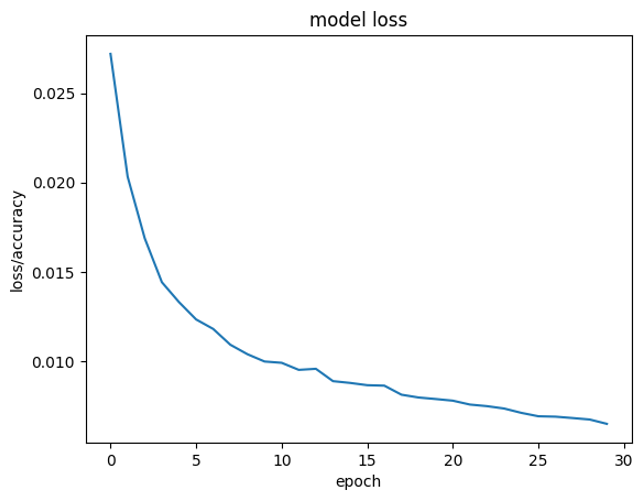
\includegraphics[width=0.7\linewidth]{gambar/bener/Loss_ModelXception.png}
	\captionof{figure}{\textit{Loss} Model CNN Xception dengan epoch 30}
	\label{fig:lossModelCNNXception}
\end{figure}

Berdasarkan Gambar \ref{fig:lossModelCNNXception}, nilai \textit{loss} pada awal pelatihan (epoch 1) cukup tinggi yaitu sekitar 0,027. Hal ini menunjukkan bahwa model asli tidak dapat memberikan prediksi yang akurat.

Namun, seiring dengan kemajuan zaman dan pendidikan, nilai \textit{loss} tersebut berangsur-angsur berkurang. Semakin kecil nilai \textit{loss}, semakin baik model mampu membuat prediksi yang mendekati nilai sebenarnya atau label yang benar.

Di akhir pelatihan (Epoch 30), nilai \textit{loss} sekitar 0,0065, menunjukkan bahwa model berhasil dipelajari dan dapat membuat prediksi yang cukup akurat.  

\begin{figure}[!hbt]
	\centering
	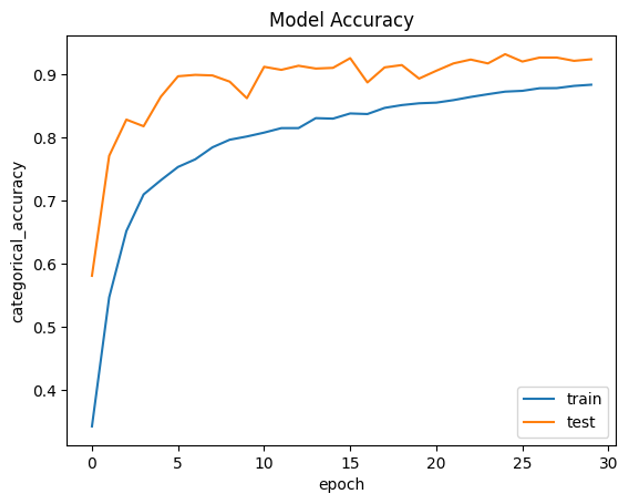
\includegraphics[width=0.7\linewidth]{gambar/bener/Accuracy_ModelXception.png}
	\captionof{figure}{Akurasi Model CNN Xception dengan epoch 30}
	\label{fig:akurasiModelCNNXception}
\end{figure}
Berdasarkan Gambar 14 , Pada awal pelatihan (Epoch 1), akurasi model relatif rendah, sekitar 34.20\%, sementara akurasi validasi sekitar 58.07\%. Ini menunjukkan bahwa model awal memiliki kinerja yang rendah dan perlu ditingkatkan.

Namun, seiring dengan berjalannya\textit{ epoch} dan pelatihan, akurasi model secara bertahap meningkat dari\textit{ epoch} ke\textit{ epoch}. Akurasi validasi juga mengalami peningkatan seiring waktu. Pada akhir pelatihan (Epoch 30), akurasi model mencapai sekitar 88.36\%, sedangkan akurasi validasi mencapai sekitar 92.39\%.

Grafik ini menggambarkan perbaikan performa model seiring berjalannya waktu. Terjadi peningkatan yang konsisten dalam akurasi model dan akurasi validasi dari\textit{ epoch} ke\textit{ epoch}.

Sebagai bagian dari pengujian fungsionalitas Model CNN Xception, dilakukan perhitungan \textit{Confusion Matrix} menggunakan dataset training sebanyak 21.600 data. \textit{Confusion Matrix} adalah sebuah matriks yang menampilkan jumlah data yang diklasifikasikan secara benar dan salah dalam setiap kelas. Detail dari \textit{Confusion Matrix} tersebut dapat ditemukan pada Gambar \ref{fig:TabelModelCNNResNet50v2}. Berdasarkan \textit{Confusion Matrix} yang dihasilkan, dilakukan perhitungan beberapa metrik evaluasi seperti \textit{F1-score}, presisi, dan \textit{recall}. Metrik-metrik evaluasi ini memberikan gambaran tentang performa dan akurasi Model CNN dalam melakukan klasifikasi.

\begin{figure}[!hbt]
	\centering
	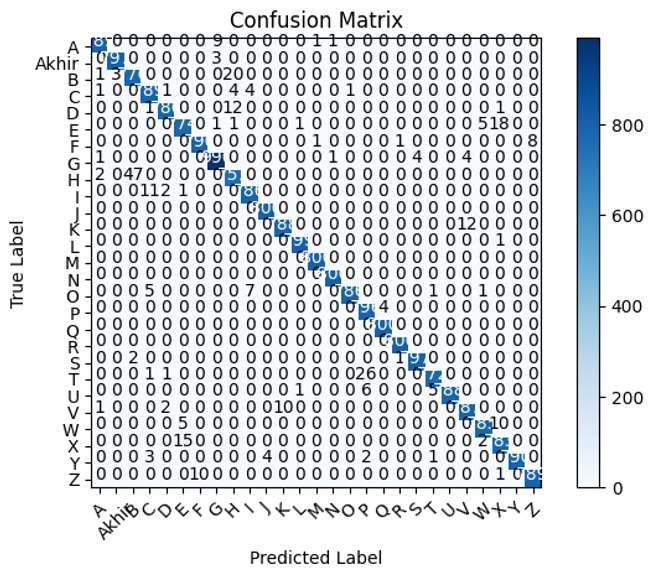
\includegraphics[width=0.7\linewidth]{gambar/bener/ConfusionMatrix_ModelXception.png}
	\captionof{figure}{Confusion Matrix Model CNN Xception dengan epoch 30}
	\label{fig:confusionmatrixModelCNNXception}
\end{figure}

Pada matriks tersebut, terdapat beberapa hasil yang perlu diperhatikan. Terlihat bahwa banyak kelas huruf yang berhasil diklasifikasikan dengan baik oleh model, seperti huruf A, Akhir, F, G, dan M, yang memiliki nilai \textit{True Positives } yang tinggi. Sebaliknya, terdapat beberapa kesalahan prediksi pada beberapa kelas huruf, seperti pada huruf B, C, D, E, H, dan I, yang memiliki beberapa False Positives dan False Negatives .

Dalam kasus ini, beberapa kelas huruf menghadapi kesulitan dalam pengklasifikasian. Sebagai contoh, huruf H dan I memiliki jumlah FP yang cukup signifikan, yang menunjukkan kesulitan model dalam membedakan antara kelas tersebut dengan kelas lainnya. Selain itu, huruf B juga mengalami kesulitan dalam pengklasifikasian, ditandai dengan jumlah FN dan FP yang lebih tinggi dibandingkan dengan kelas huruf lainnya.

Selain itu, terdapat pula beberapa kesalahan yang terjadi dalam prediksi. Misalnya, pada baris A dan kolom G, terdapat 9 contoh yang salah terklasifikasi sebagai huruf G, sedangkan pada baris G dan kolom A, terdapat 4 contoh yang salah terklasifikasi sebagai huruf A.

Berikut merupakan tabel perhitungan \textit{F1-score}, presisi, dan recall yang dapat dilihat pada Tabel \ref{tbl:Tabel Confusion Matrix Xception} \textit{Xception} menggunakan \textit{Confusion Matrix} pada Gambar \ref{fig:confusionmatrixModelCNNXception}.

\begin{center}
	\begin{table}[!hbt]
	\centering
	\captionof{table}{Tabel Confusion Matrix \textit{ Xception}}
	\label{tbl:Tabel Confusion Matrix Xception}
	\begin{tabular}{|c|c|c|c|c|}
	\hline
	Class & Precision & Recall & F1-score & Accuracy \\
	\hline
	A & 0.9925 & 0.9863 & 0.9893 & 0.9863 \\
	Akhir & 0.9963 & 0.9963 & 0.9963 & 0.9963 \\
	B & 0.9406 & 0.9700 & 0.9551 & 0.9700 \\
	C & 0.9741 & 0.9863 & 0.9801 & 0.9863 \\
	D & 0.9924 & 0.9825 & 0.9874 & 0.9825 \\
	E & 0.9736 & 0.9675 & 0.9705 & 0.9675 \\
	F & 0.9875 & 0.9875 & 0.9875 & 0.9875 \\
	G & 0.9870 & 0.9900 & 0.9885 & 0.9900 \\
	H & 0.9530 & 0.9388 & 0.9458 & 0.9388 \\
	I & 0.9862 & 0.9825 & 0.9843 & 0.9825 \\
	J & 0.9950 & 1.0000 & 0.9975 & 1.0000 \\
	K & 0.9875 & 0.9850 & 0.9862 & 0.9850 \\
	L & 0.9975 & 0.9988 & 0.9981 & 0.9988 \\
	M & 0.9975 & 1.0000 & 0.9988 & 1.0000 \\
	N & 0.9975 & 1.0000 & 0.9988 & 1.0000 \\
	O & 0.9987 & 0.9825 & 0.9905 & 0.9825 \\
	P & 0.9590 & 0.9950 & 0.9767 & 0.9950 \\
	Q & 0.9950 & 1.0000 & 0.9975 & 1.0000 \\
	R & 0.9975 & 1.0000 & 0.9988 & 1.0000 \\
	S & 0.9950 & 0.9963 & 0.9956 & 0.9963 \\
	T & 0.9910 & 0.9650 & 0.9778 & 0.9650 \\
	U & 1.0000 & 0.9850 & 0.9924 & 0.9850 \\
	V & 0.9801 & 0.9838 & 0.9819 & 0.9838 \\
	W & 0.9899 & 0.9813 & 0.9856 & 0.9813 \\
	X & 0.9619 & 0.9788 & 0.9703 & 0.9788 \\
	Y & 1.0000 & 0.9875 & 0.9937 & 0.9875 \\
	Z & 0.9900 & 0.9863 & 0.9881 & 0.9863 \\
	\hline
	\end{tabular}
\end{table}
\end{center}

Berdasarkan \ref{tbl:Tabel Confusion Matrix Xception} , Rata-rata \textit{Precision}, Recall, \textit{F1-Score}, dan \textit{Accuracy} dari model CNN yang dihasilkan dapat memberikan gambaran tentang kinerja keseluruhan model dalam mengklasifikasikan huruf dan kata yang diuji. Dari analisis tabel, ditemukan bahwa rata-rata \textit{Precision} sebesar 98.77\%, yang menunjukkan bahwa model memiliki kemampuan yang baik dalam mengidentifikasi kelas dengan benar. Selain itu, rata-rata Recall sebesar 98.72\% mengindikasikan kemampuan model dalam menemukan kembali sampel positif dari suatu kelas. Rata-rata \textit{F1-Score} sebesar 98.73\% menggambarkan keseimbangan antara \textit{Precision} dan Recall, menghasilkan pengukuran keseluruhan yang baik. Terakhir, rata-rata \textit{Accuracy} sebesar 98.78\% menunjukkan tingkat keseluruhan ketepatan model dalam mengklasifikasikan keseluruhan sampel dengan benar.


\section{Hasil Waktu Pelatihan}
Selain mendapatkan nilai akurasi , \textit{loss} , tabel \textit{Confusion Matrix} , \textit{F1-Score} , Recall maupun Presisi . Di dalam penelitian ini juga didapatkan hasil dari lama waktu selama melakukan pelatihan model berbagai macam skenario dari setiap \textit{ epoch} yang berhasil dilewati 

Berikut ini merupakan tabel yang memaparkan informasi terkait lama waktu pelatihan model per\textit{ epoch} dari masing-masing skenario yang telah diujicoba 

\begin{table}[!hbt]
	\centering
	\captionof{table}{Durasi Pelatihan dalam detik untuk Epoch 1-30}
	\label{tab:training_time}
	\begin{tabular}{|c|c|c|c|c|} 
	\hline
	Epoch & CNN & CNN2 & Xception & ResNet50V2\\
	\hline
	1              & 18.89        & 19.64         & 212.01            & 200.52              \\
	2              & 19.14        & 19.39         & 204.80            & 208.99              \\
	3              & 18.99        & 18.83         & 210.35            & 201.25              \\
	4              & 18.86        & 19.78         & 214.80            & 191.17              \\
	5              & 19.14        & 20.40         & 201.79            & 195.61              \\
	6              & 20.20        & 20.12         & 202.45            & 192.91              \\
	7              & 19.83        & 19.97         & 198.41            & 192.96              \\
	8              & 21.73        & 19.28         & 192.45            & 191.49              \\
	9              & 20.27        & 20.17         & 189.75            & 196.54              \\
	10             & 19.94        & 20.77         & 188.84            & 199.96              \\
	11             & 20.97        & 21.56         & 189.66            & 195.11              \\
	12             & 21.17        & 20.56         & 187.79            & 188.70              \\
	13             & 21.55        & 20.19         & 188.07            & 189.04              \\
	14             & 21.36        & 20.55         & 185.68            & 224.72              \\
	15             & 21.19        & 19.37         & 184.83            & 208.74              \\
	16             & 21.02        & 20.11         & 185.04            & 217.11              \\
	17             & 21.24        & 20.80         & 188.87            & 204.28              \\
	18             & 21.51        & 19.41         & 190.76            & 224.57              \\
	19             & 21.45        & 19.78         & 193.68            & 204.64              \\
	20             & 21.79        & 19.77         & 193.92            & 181.35              \\
	21             & 20.57        & 19.80         & 186.56            & 175.74              \\
	22             & 21.11        & 20.40         & 185.24            & 180.82              \\
	23             & 21.48        & 20.14         & 185.09            & 173.18              \\
	24             & 21.00        & 20.09         & 186.67            & 163.73              \\
	25             & 21.90        & 20.12         & 185.66            & 168.90              \\
	26             & 23.09        & 20.31         & 185.45            & 164.35              \\
	27             & 22.81        & 19.69         & 184.81            & 164.39              \\
	28             & 23.44        & 19.10         & 185.45            & 163.14              \\
	29             & 22.45        & 19.27         & 187.25            & 161.36              \\
	30             & 22.35        & 19.54         & 187.09            & 162.61              \\ 
	\hline
	\end{tabular}
\end{table}

Berdasarkan tabel di atas, dapat dilihat bahwa Model CNN memiliki waktu pelatihan yang relatif stabil selama 30\textit{ epoch}, dengan rata-rata waktu pelatihan sekitar 19-22 detik per\textit{ epoch}. Model CNN2 juga memiliki pola waktu pelatihan yang serupa, dengan rata-rata waktu pelatihan sekitar 19-21 detik per\textit{ epoch}.

Di sisi lain, Model \textit{Xception} dan Model \textit{ResNet50V2 }memiliki waktu pelatihan yang lebih lama secara signifikan. Model \textit{Xception} membutuhkan waktu pelatihan sekitar 185-213 detik per\textit{ epoch}, sementara Model \textit{ResNet50V2 }membutuhkan waktu pelatihan sekitar 163-225 detik per\textit{ epoch}.
	
Dapat disimpulkan bahwa Model CNN dan Model CNN2 memiliki waktu pelatihan yang lebih efisien dibandingkan dengan Model \textit{Xception} dan Model ResNet50V2. Ini mungkin dikaitkan dengan perbedaan arsitektur dan kompleksitas model tersebut. Model CNN dan CNN2 mungkin lebih sederhana dan memiliki jumlah parameter yang lebih sedikit dibandingkan dengan \textit{Xception} dan ResNet50V2, sehingga memungkinkan pelatihan yang lebih cepat.

\section{Ujicoba Deteksi}
Dalam bagian ini , Telah dilakukan ujicoba perangkat lunak yang sudah dibuat dengan cara melakukan ujicoba langsung kepada orang yang mencoba . Dalam ujicoba kali ini diberikan contoh deteksi huruf vokal yaitu A,I,U,E,O dan membentuk kata seperti Bapak , Ibu dan Tante . Ujicoba ini dilakukan terhadap dua orang dengan mengambil jarak 100 cm dari Kamera

\subsection{Orang Pertama}
Pada tahap ujicoba ini, telah dilakukan serangkaian percobaan menggunakan beberapa model CNN yang berbeda, yaitu Model CNN, Model CNN2, Model CNN ResNet50V2, dan Model CNN Xception. Ujicoba tersebut bertujuan untuk menguji kemampuan dan kinerja masing-masing model dalam mengenali huruf serta merangkainya menjadi kata-kata. Dalam setiap percobaan, orang pertama telah menjadi subjek yang diuji dengan menggunakan model-model tersebut. 

Hasil ujicoba akan memberikan pemahaman yang lebih mendalam tentang keefektifan dan kehandalan masing-masing model dalam mengenali dan mengolah huruf-huruf menjadi kata-kata 

\subsubsection*{Hasil Model CNN Orang Pertama}

Setelah melalui serangkaian ujicoba, ModelCNN telah menunjukkan kinerjanya yang luar biasa dalam melakukan deteksi huruf dengan tingkat keberhasilan yang sangat baik. Salah satu kemampuan utamanya adalah mampu mengenali huruf-huruf dengan akurasi yang tinggi, bahkan dalam berbagai posisi dan pose yang berbeda

\begin{table}[!hbt]
	\centering
	\captionof{table}{Tabel Contoh Huruf/Kata dan Gambar Pose Model CNN Orang Pertama}
	\label{tbl:Tabel Contoh Huruf/Kata dan Gambar Pose Model CNN Orang Pertama}
	\begin{tabular}{|c|c|c|}
	\hline
	No & Huruf/Kata & Gambar Pose Model CNN \\
	\hline
	1 & A & 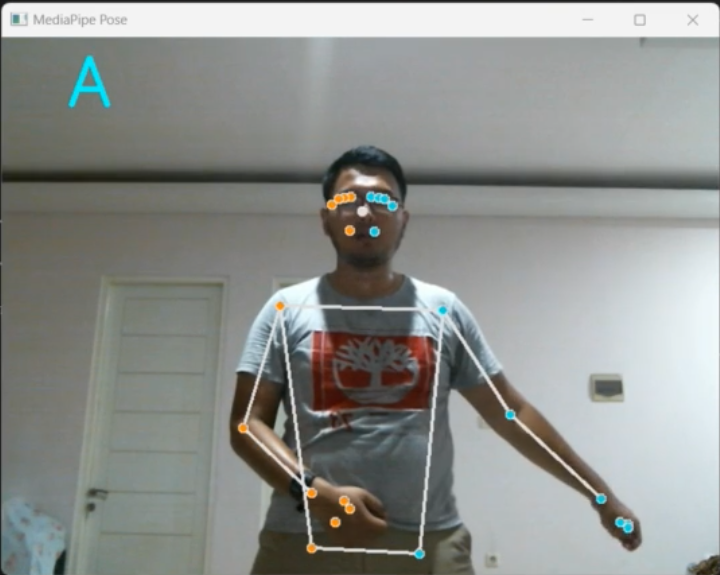
\includegraphics[width=0.2\textwidth]{gambar/bener/HurufA_ModelCNN_Dawe.png} \\
	\hline
	2 & I & 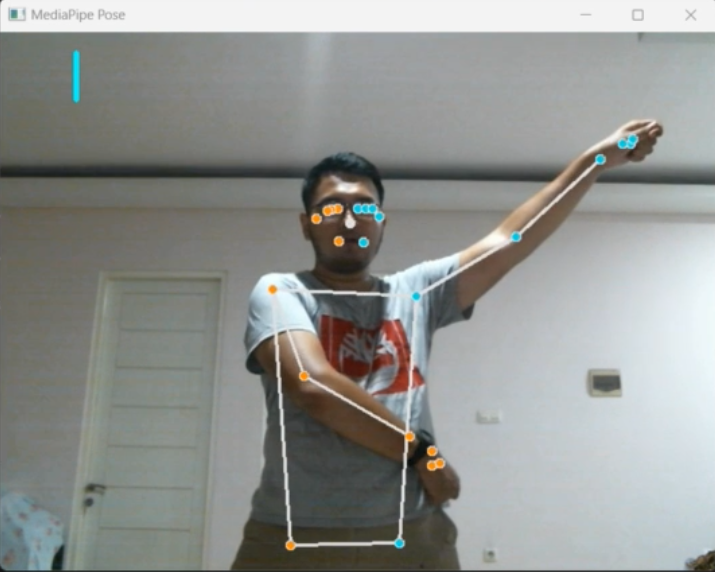
\includegraphics[width=0.2\textwidth]{gambar/bener/HurufI_ModelCNN_Dawe.png} \\
	\hline
	3 & U & 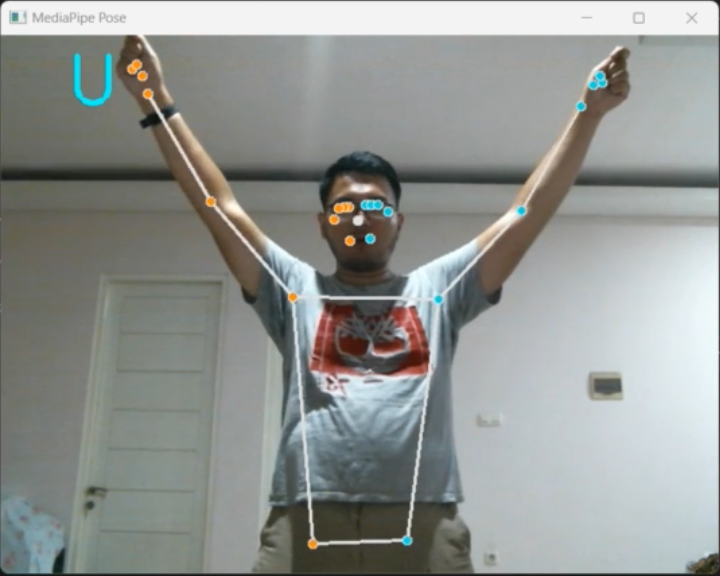
\includegraphics[width=0.2\textwidth]{gambar/bener/HurufU_ModelCNN_Dawe.png} \\
	\hline
	4 & E & 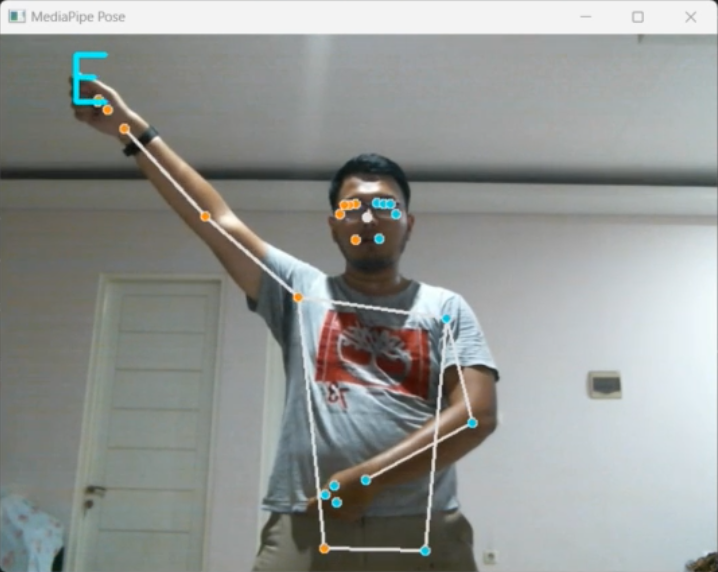
\includegraphics[width=0.2\textwidth]{gambar/bener/HurufE_ModelCNN_Dawe.png} \\
	\hline
	5 & O & 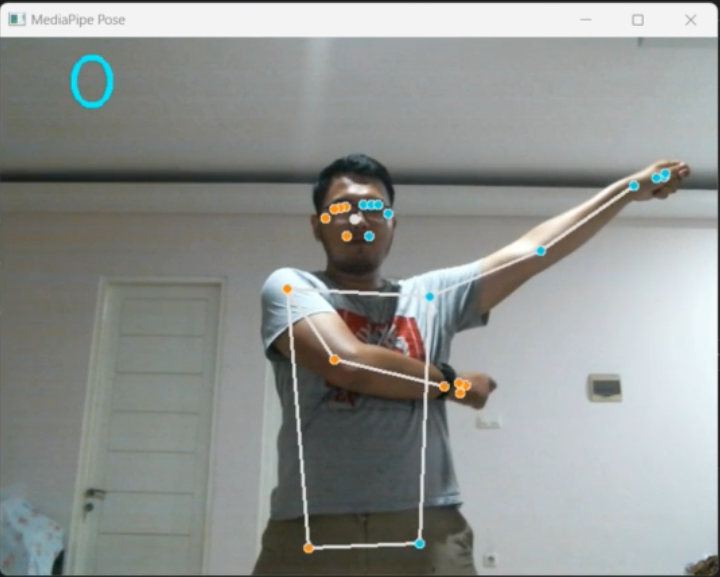
\includegraphics[width=0.2\textwidth]{gambar/bener/HurufO_ModelCNN_Dawe.png} \\
	\hline
	6 & B & 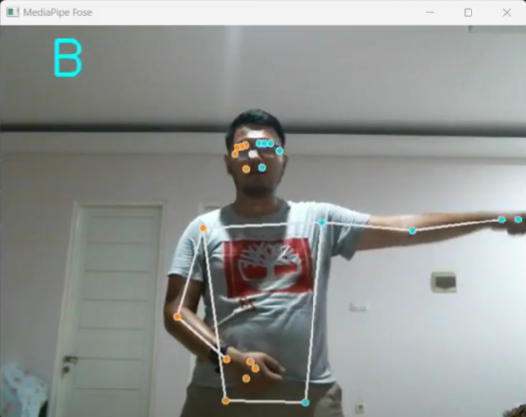
\includegraphics[width=0.2\textwidth]{gambar/bener/HurufB_ModelCNN_Dawe.png} \\
	\hline
	7 & K & 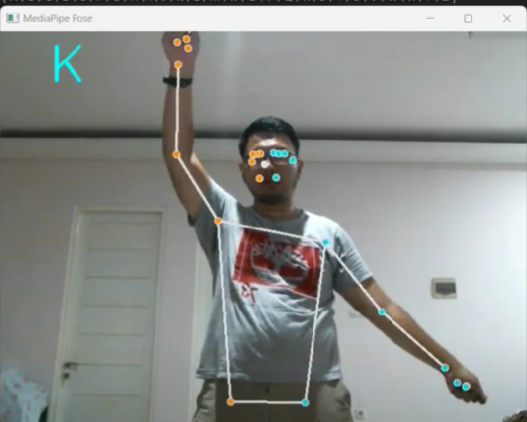
\includegraphics[width=0.2\textwidth]{gambar/bener/HurufK_ModelCNN_Dawe.png} \\
	\hline
	8 & H & 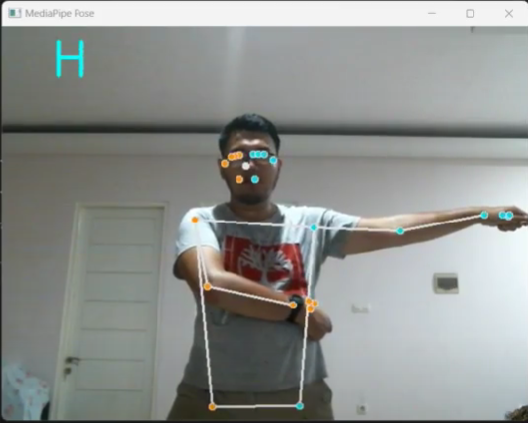
\includegraphics[width=0.2\textwidth]{gambar/bener/HurufH_ModelCNN_Dawe.png} \\
	\hline
	% Lanjutkan baris tabel sesuai kebutuhan
	\end{tabular}
\end{table}

\begin{table}[!hbt]
	\centering
	\captionof{table}{Tabel Contoh Huruf/Kata dan Gambar Pose Model CNN Orang Pertama}
	\begin{tabular}{|c|c|c|}
		\hline
		No & Huruf/Kata & Gambar Pose Model  \\
		\hline
		9 & Bapak & 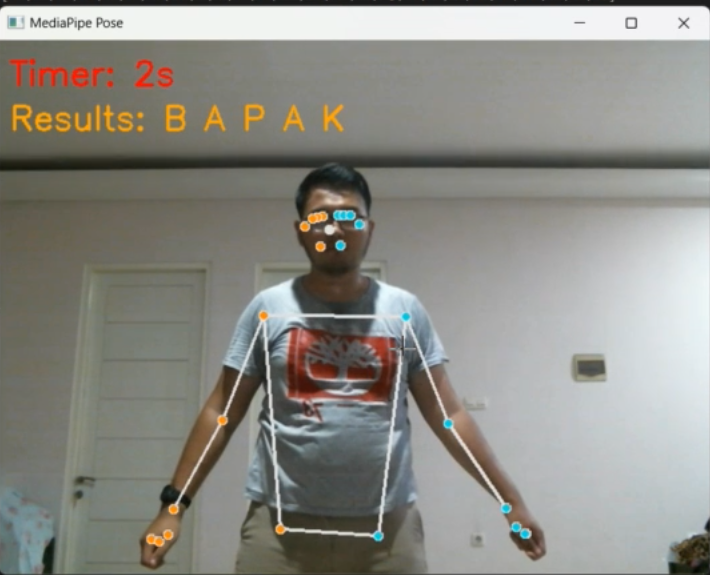
\includegraphics[width=0.2\textwidth]{gambar/bener/HurufBapak_ModelCNN_Dawe.png} \\
		\hline
		10 & Ibu & 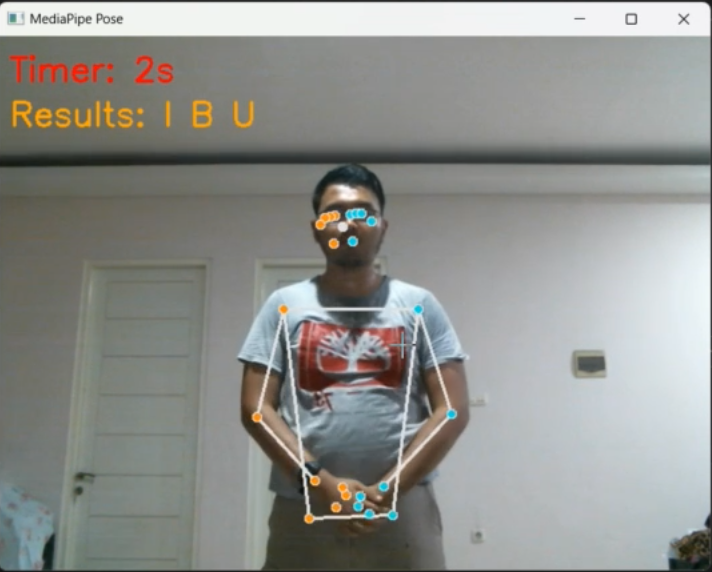
\includegraphics[width=0.2\textwidth]{gambar/bener/HurufIbu_ModelCNN_Dawe.png} \\
		\hline
		11 & Tante & 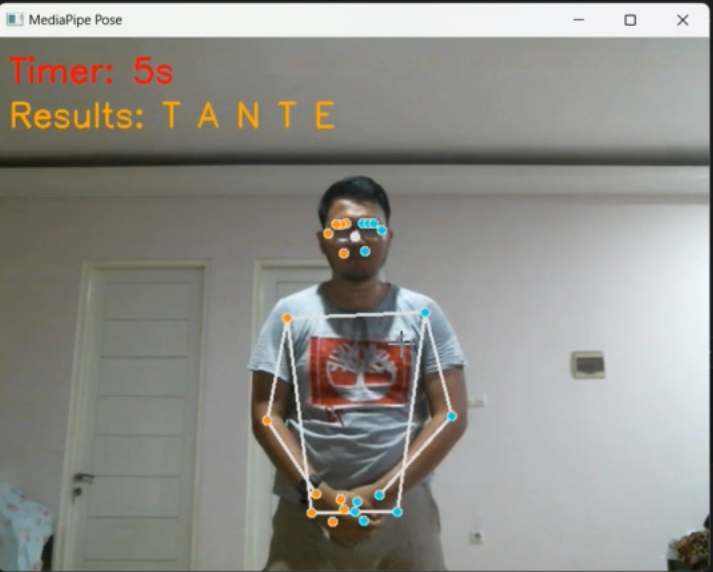
\includegraphics[width=0.2\textwidth]{gambar/bener/HurufTante_ModelCNN_Dawe.png} \\
		\hline
	\end{tabular}
\end{table}

\subsubsection*{Hasil Model CNN2 Orang Pertama}

Dari hasil ujicoba yang dilakukan, ModelCNN2 telah berhasil dalam melakukan deteksi dengan tingkat keberhasilan yang baik. Salah satu kemampuan utama model ini adalah mampu mendeteksi huruf-huruf dengan akurasi yang tinggi

\begin{table}[!hbt]
	\centering
	\captionof{table}{Tabel Contoh Huruf/Kata dan Gambar Pose Model CNN2 Orang Pertama}
	\label{tbl:Tabel Contoh Huruf/Kata dan Gambar Pose Model CNN2 Orang Pertama}
	\begin{tabular}{|c|c|c|}
	\hline
	No & Huruf/Kata & Gambar Pose Model  \\
	\hline
	1 & A & 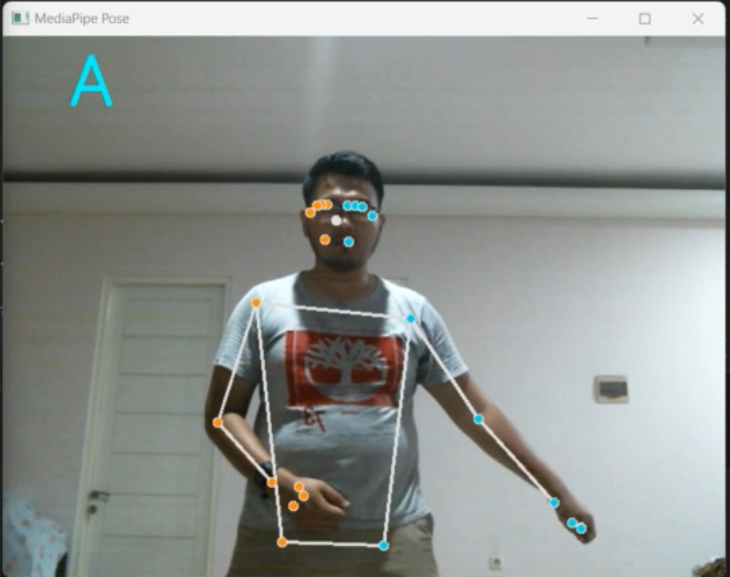
\includegraphics[width=0.2\textwidth]{gambar/bener/HurufA_ModelCNN2_Dawe.png} \\
	\hline
	2 & I & 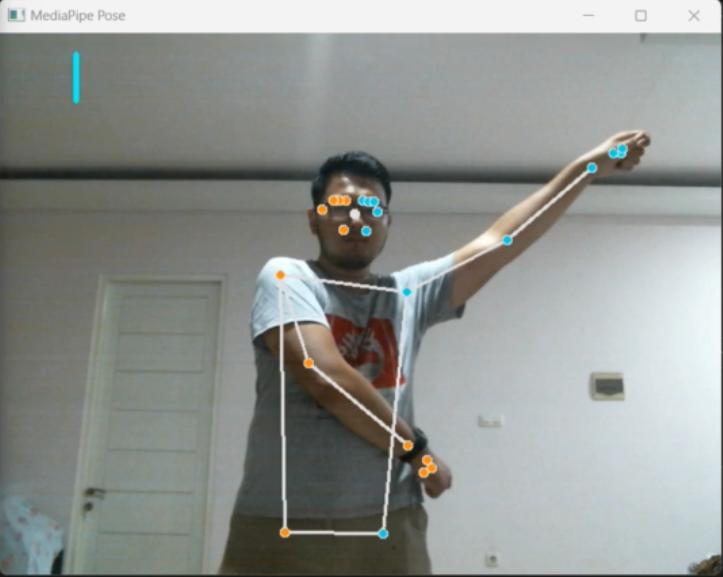
\includegraphics[width=0.2\textwidth]{gambar/bener/HurufI_ModelCNN2_Dawe.png} \\
	\hline
	3 & U & 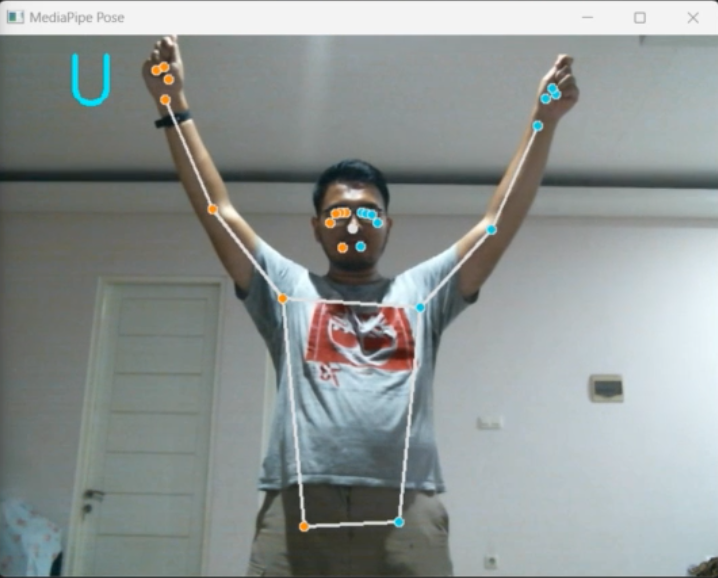
\includegraphics[width=0.2\textwidth]{gambar/bener/HurufU_ModelCNN2_Dawe.png} \\
	\hline
	4 & E & 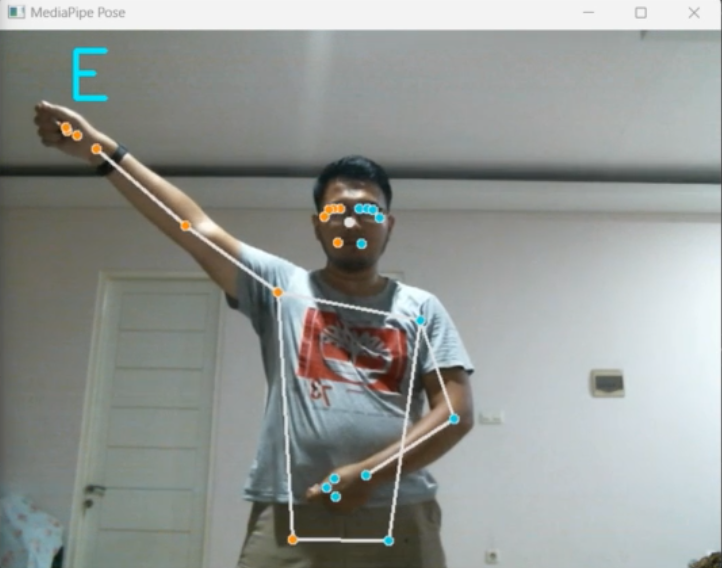
\includegraphics[width=0.2\textwidth]{gambar/bener/HurufE_ModelCNN2_Dawe.png} \\
	\hline
	5 & O & 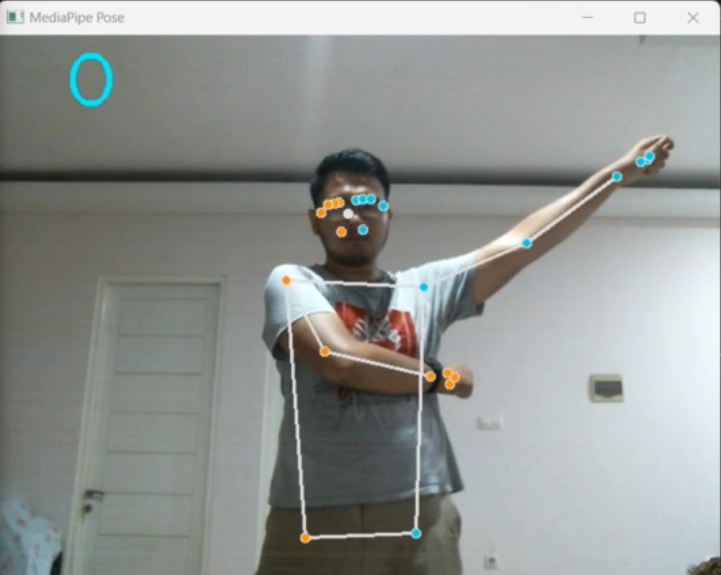
\includegraphics[width=0.2\textwidth]{gambar/bener/HurufO_ModelCNN2_Dawe.png} \\
	\hline
	6 & B & 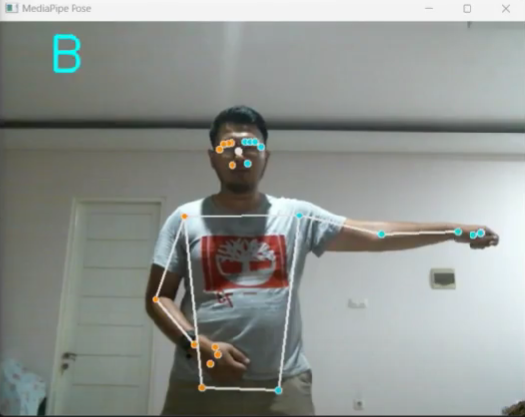
\includegraphics[width=0.2\textwidth]{gambar/bener/HurufB_ModelCNN2_Dawe.png} \\
	\hline
	7 & K & 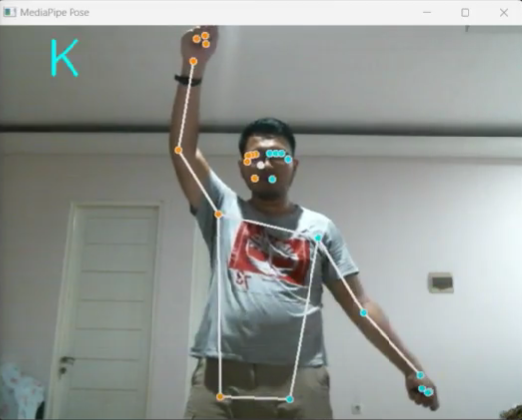
\includegraphics[width=0.2\textwidth]{gambar/bener/HurufK_ModelCNN2_Dawe.png} \\
	\hline
	8 & H & 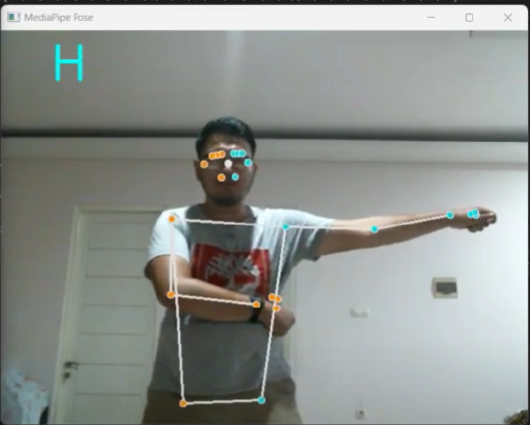
\includegraphics[width=0.2\textwidth]{gambar/bener/HurufH_ModelCNN2_Dawe.png} \\
	\hline
	% Lanjutkan baris tabel sesuai kebutuhan
	\end{tabular}
\end{table}

\begin{table}[!hbt]
	\centering
	\captionof{table}{Tabel Contoh Huruf/Kata dan Gambar Pose Model CNN2 Orang Pertama}
	\begin{tabular}{|c|c|c|}
		\hline
		No & Huruf/Kata & Gambar Pose Model  \\
		\hline
		9 & Bapak & 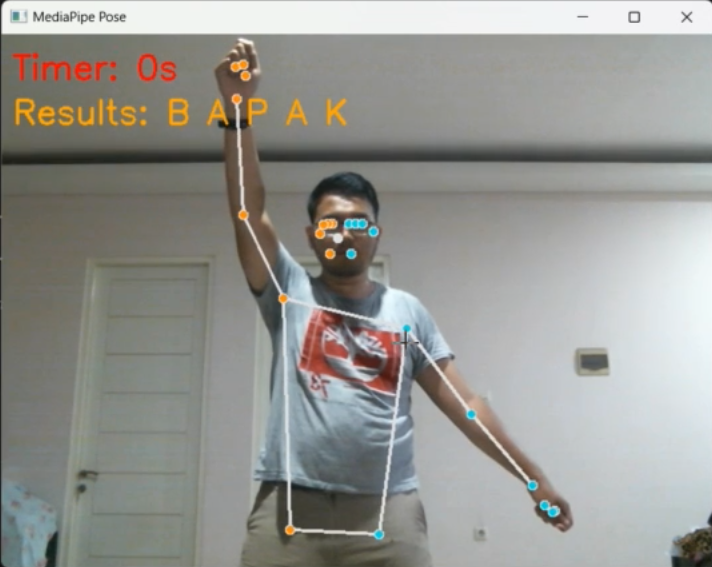
\includegraphics[width=0.2\textwidth]{gambar/bener/HurufBapak_CNN2_Dawe.png} \\
		\hline
		10 & Ibu & 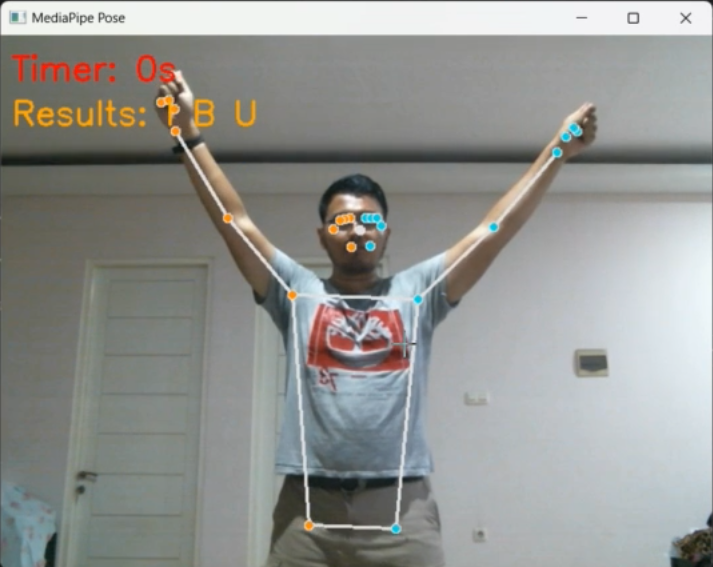
\includegraphics[width=0.2\textwidth]{gambar/bener/HurufIbu_ModelCNN2_Dawe.png} \\
		\hline
		11 & Tante & 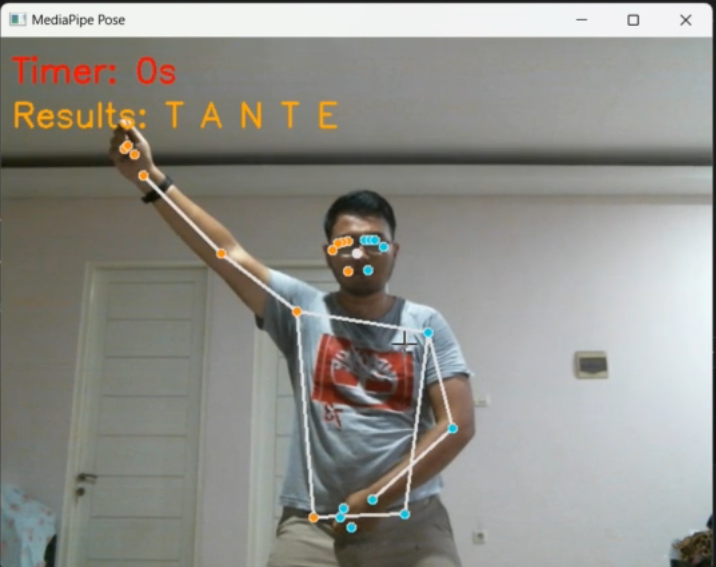
\includegraphics[width=0.2\textwidth]{gambar/bener/HurufTante_ModelCNN2_Dawe.png} \\
		\hline
	\end{tabular}
\end{table}

\subsubsection*{Hasil Model CNN \textit{ResNet50V2 }Orang Pertama}

Berdasarkan hasil ujicoba yang dilakukan, ModelCNN \textit{ResNet50V2 }telah menunjukkan kemampuannya yang sangat baik dalam melakukan deteksi huruf dengan tingkat keberhasilan yang tinggi. Salah satu keunggulan utama dari model ini adalah kemampuannya untuk mendeteksi huruf dengan akurat, bahkan dalam pose yang bervariasi. Dalam ujicoba tersebut, ModelCNN \textit{ResNet50V2 }berhasil mengatasi tantangan yang mungkin muncul akibat perubahan pose huruf, sehingga dapat mengenali huruf-huruf dengan presisi yang memuaskan

\begin{table}[!hbt]
	\centering
	\captionof{table}{Tabel Contoh Huruf/Kata dan Gambar Pose Model CNN \textit{ResNet50V2 }Orang Pertama}
	\label{tbl:Tabel Contoh Huruf/Kata dan Gambar Pose Model CNN ResNet50V2 Orang Pertama}
	\begin{tabular}{|c|c|c|}
	\hline
	No & Huruf/Kata & Gambar Pose Model  \\
	\hline
	1 & A & 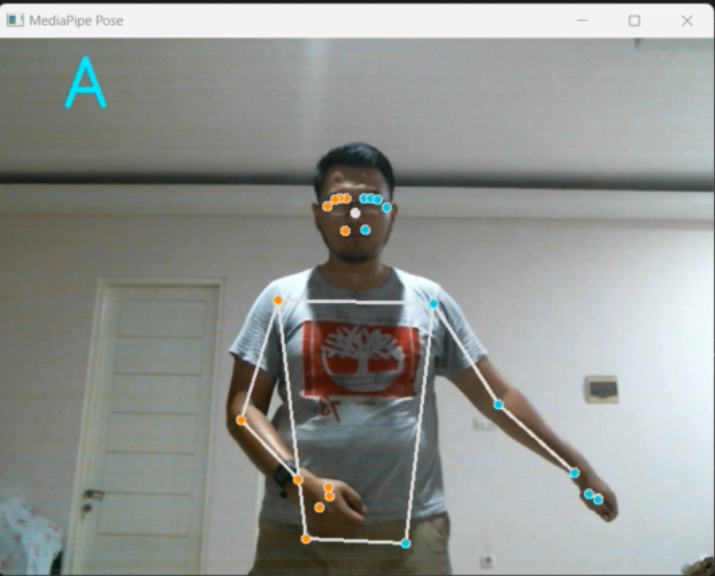
\includegraphics[width=0.2\textwidth]{gambar/bener/HurufA_ModelCNNResNet50V2_Dawe.png} \\
	\hline
	2 & I & 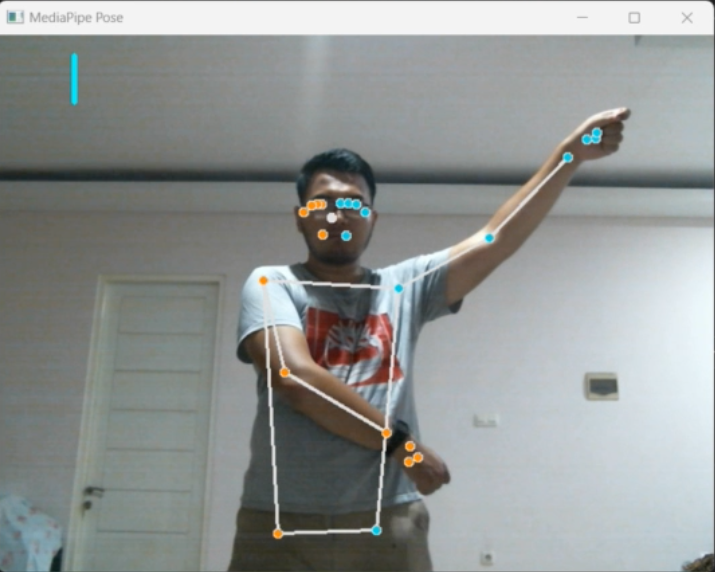
\includegraphics[width=0.2\textwidth]{gambar/bener/HurufI_ModelCNNResNet50V2_Dawe.png} \\
	\hline
	3 & U & 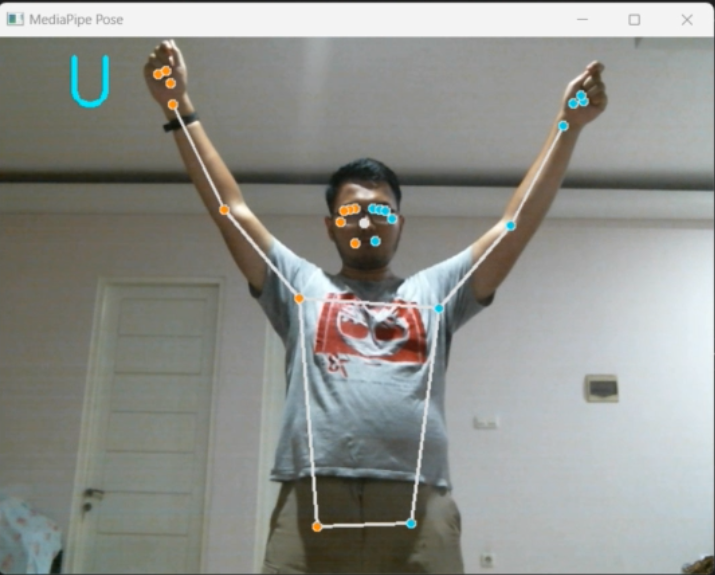
\includegraphics[width=0.2\textwidth]{gambar/bener/HurufU_ModelCNNResNet50V2_Dawe.png} \\
	\hline
	4 & E & 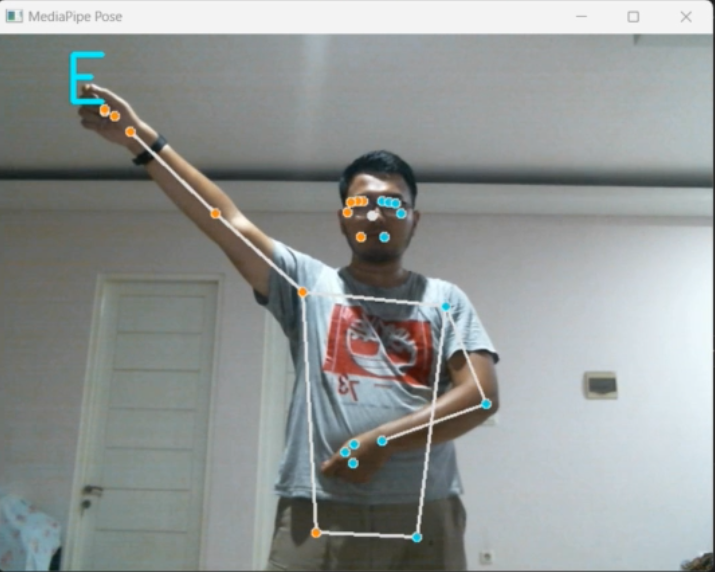
\includegraphics[width=0.2\textwidth]{gambar/bener/HurufE_ModelCNNResNet50V2_Dawe.png} \\
	\hline
	5 & O & 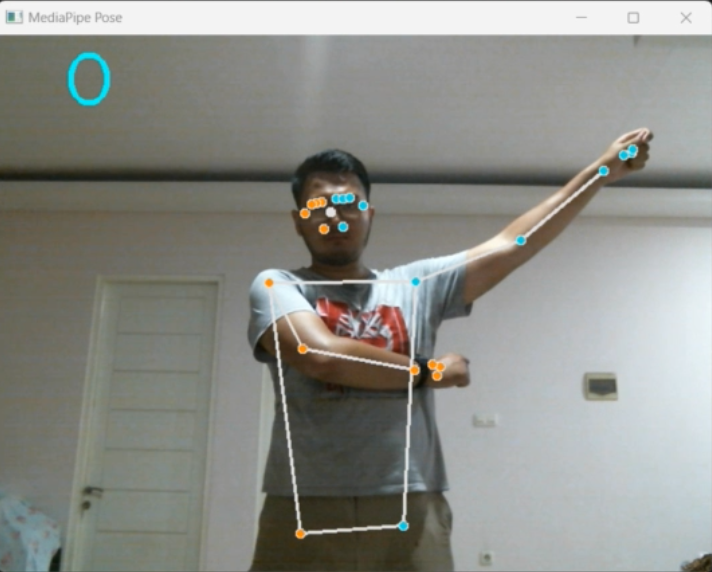
\includegraphics[width=0.2\textwidth]{gambar/bener/HurufO_ModelCNNResNet50V2_Dawe.png} \\
	\hline
	6 & B & 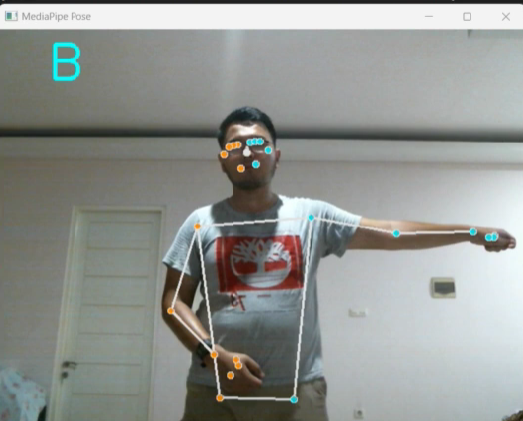
\includegraphics[width=0.2\textwidth]{gambar/bener/HurufB_ModelCNNResNet50V2_Dawe.png} \\
	\hline
	7 & K & 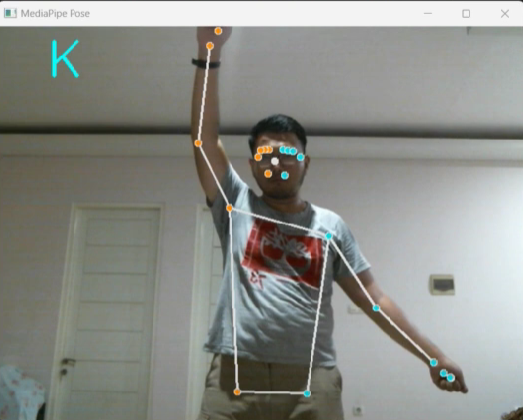
\includegraphics[width=0.2\textwidth]{gambar/bener/HurufK_ModelCNNResNet50V2_Dawe.png} \\
	\hline
	8 & H & 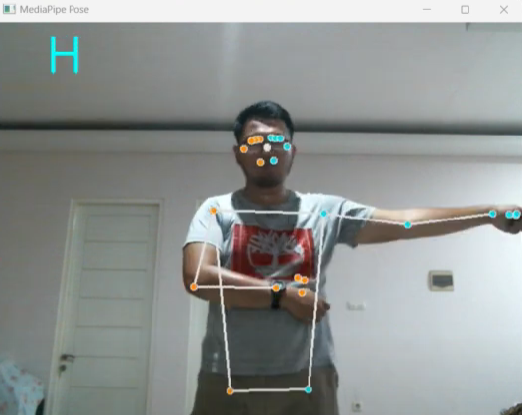
\includegraphics[width=0.2\textwidth]{gambar/bener/HurufH_ModelCNNResNet50V2_Dawe.png} \\
	\hline
	% Lanjutkan baris tabel sesuai kebutuhan
	\end{tabular}
\end{table}


\subsubsection*{Hasil Model CNN \textit{Xception} Orang Pertama}
Berdasarkan eksperimen yang dilakukan, ModelCNN \textit{Xception} telah berhasil dalam melakukan deteksi huruf dengan tingkat keberhasilan yang tinggi. Salah satu keunggulan utama dari model ini adalah kemampuannya dalam mengenali huruf dengan akurasi yang baik, bahkan ketika huruf tersebut berada dalam pose yang berbeda. Ujicoba tersebut telah menunjukkan bahwa ModelCNN \textit{Xception} mampu mengatasi tantangan yang mungkin muncul akibat variasi pose huruf, sehingga memberikan hasil yang akurat dalam pengenalan huruf

\begin{table}[!hbt]
	\centering
	\captionof{table}{Tabel Contoh Huruf/Kata dan Gambar Pose Model CNN Xception Orang Pertama}
	\label{tbl:Tabel Contoh Huruf/Kata dan Gambar Pose Model CNN Xception Orang Pertama}
	\begin{tabular}{|c|c|c|}
	\hline
	No & Huruf/Kata & Gambar Pose Model  \\
	\hline
	1 & A & 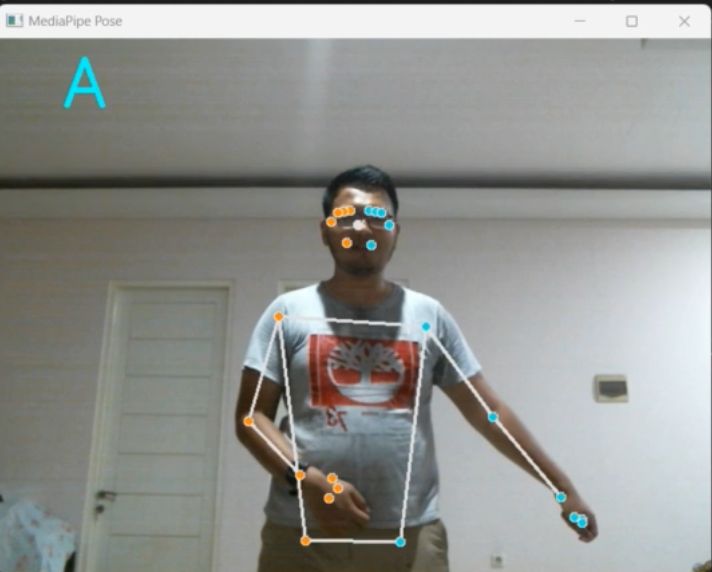
\includegraphics[width=0.2\textwidth]{gambar/bener/HurufA_ModelCNNXception_Dawe.png} \\
	\hline
	2 & I & 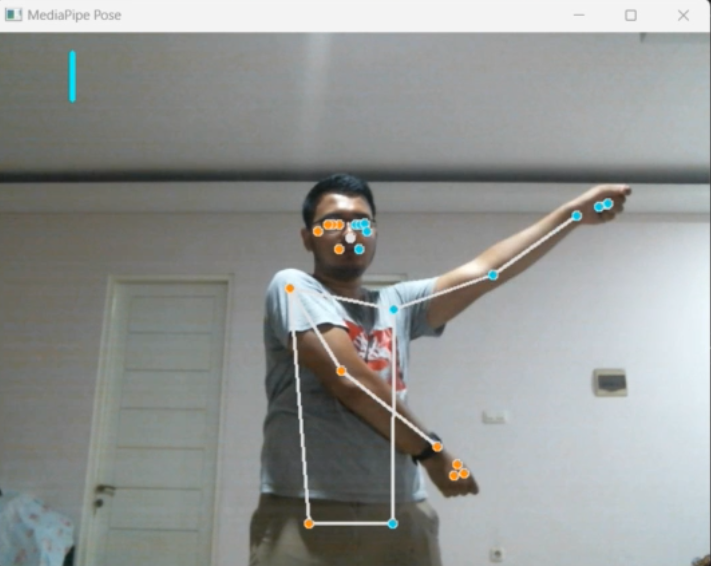
\includegraphics[width=0.2\textwidth]{gambar/bener/HurufI_ModelCNNXception_Dawe.png} \\
	\hline
	3 & U & 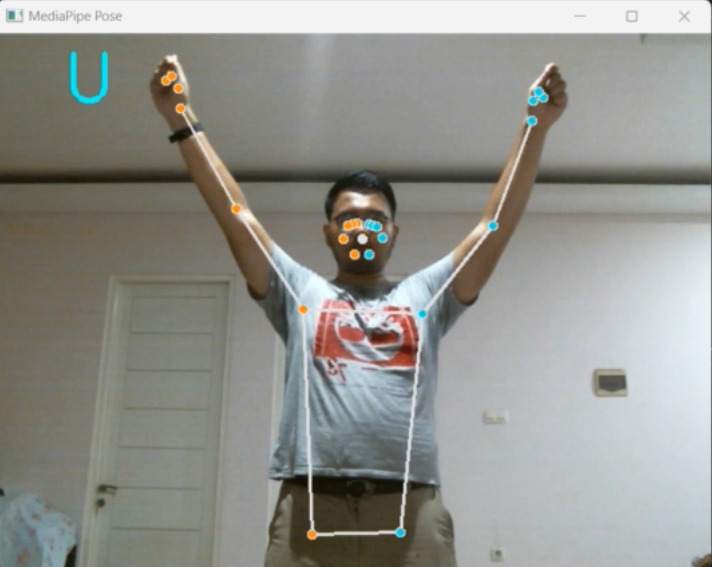
\includegraphics[width=0.2\textwidth]{gambar/bener/HurufU_ModelCNNXception_Dawe.png} \\
	\hline
	4 & E & 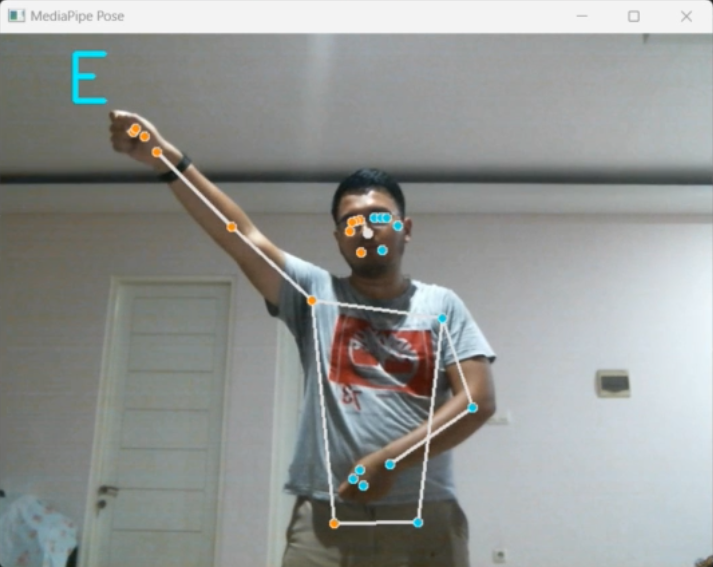
\includegraphics[width=0.2\textwidth]{gambar/bener/HurufE_ModelCNNXception_Dawe.png} \\
	\hline
	5 & O & 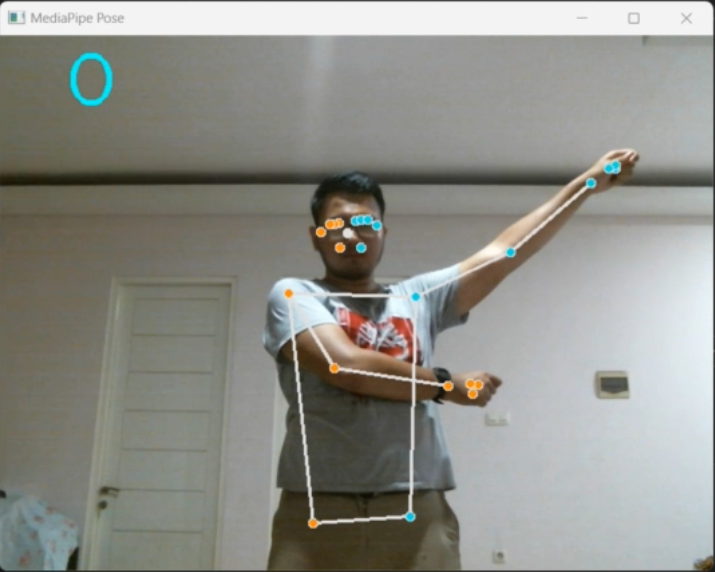
\includegraphics[width=0.2\textwidth]{gambar/bener/HurufO_ModelCNNXception_Dawe.png} \\
	\hline
	6 & B & 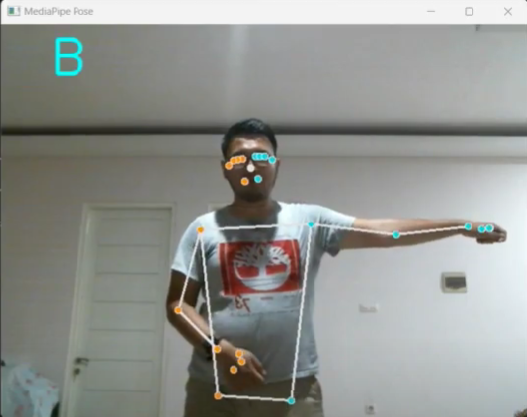
\includegraphics[width=0.2\textwidth]{gambar/bener/HurufB_ModelCNNXception_Dawe.png} \\
	\hline
	7 & K & \includegraphics[width=0.2\textwidth]{gambar/bener/HurufK_ModelCNNXception_Dawe.png} \\
	\hline
	8 & H & \includegraphics[width=0.2\textwidth]{gambar/bener/HurufH_ModelCNNXception_Dawe.png} \\
	\hline
	% Lanjutkan baris tabel sesuai kebutuhan
	\end{tabular}
\end{table}


\subsection{Orang Kedua}

Dalam serangkaian ujicoba ini, dilakukan pengujian terhadap seorang subjek kedua menggunakan beberapa model CNN yang berbeda, seperti Model CNN, Model CNN2, Model CNN ResNet50V2, dan Model CNN Xception. Ujicoba ini dilakukan dengan tujuan untuk mengevaluasi kemampuan masing-masing model dalam mengenali huruf dan membentuk kata.

Subjek kedua menjadi partisipan yang diuji dalam setiap percobaan menggunakan model-model tersebut. Melalui ujicoba ini, diharapkan dapat diperoleh pemahaman yang lebih mendalam mengenai keefektifan dan keandalan setiap model dalam pengenalan huruf dan pembentukan kata-kata

\subsubsection*{Hasil Model CNN Orang Kedua}

Berdasarkan percobaan yang dilakukan, ModelCNN telah menunjukkan kemampuannya yang baik dalam mengenali dan mendeteksi huruf dengan akurasi yang memuaskan.

\begin{table}[!hbt]
	\centering
	\captionof{table}{Tabel Contoh Huruf/Kata dan Gambar Pose Model CNN}
	\label{tbl:Tabel Contoh Huruf/Kata dan Gambar Pose Model CNN Orang Kedua}
	\begin{tabular}{|c|c|c|}
	\hline
	No & Huruf/Kata & Gambar Pose Model CNN \\
	\hline
	1 & A & \includegraphics[width=0.2\textwidth]{gambar/bener/HurufA_ModelCNN_Fachry.png} \\
	\hline
	2 & I & \includegraphics[width=0.2\textwidth]{gambar/bener/HurufI_ModelCNN_Fachry.png} \\
	\hline
	3 & U & \includegraphics[width=0.2\textwidth]{gambar/bener/HurufU_ModelCNN_Fachry.png} \\
	\hline
	4 & E & \includegraphics[width=0.2\textwidth]{gambar/bener/HurufE_ModelCNN_Fachry.png} \\
	\hline
	5 & O & \includegraphics[width=0.2\textwidth]{gambar/bener/HurufO_ModelCNN_Fachry.png} \\
	\hline
	6 & B & \includegraphics[width=0.2\textwidth]{gambar/bener/HurufB_ModelCNN_Fachry.png} \\
	\hline
	7 & K & \includegraphics[width=0.2\textwidth]{gambar/bener/HurufK_ModelCNN_Fachry.png} \\
	\hline
	8 & H & \includegraphics[width=0.2\textwidth]{gambar/bener/HurufH_ModelCNN_Fachry.png} \\
	\hline
	% Lanjutkan baris tabel sesuai kebutuhan
	\end{tabular}
	\end{table}

\begin{table}[!hbt]
	\centering
	\captionof{table}{Tabel Contoh Huruf/Kata dan Gambar Pose Model CNN2}
	\begin{tabular}{|c|c|c|}
		\hline
		No & Huruf/Kata & Gambar Pose Model  \\
		\hline
		9 & Bapak & \includegraphics[width=0.2\textwidth]{gambar/bener/HurufBapak_ModelCNN_Fachry.png} \\
		\hline
		10 & Ibu & \includegraphics[width=0.2\textwidth]{gambar/bener/HurufIbu_ModelCNN_Fachry.png} \\
		\hline
		11 & Tante & \includegraphics[width=0.2\textwidth]{gambar/bener/HurufTante_ModelCNN_Fachry.png} \\
		\hline
	\end{tabular}
\end{table}

\subsubsection*{Hasil Model CNN2 Orang Kedua}

Hasil ujicoba menunjukkan bahwa ModelCNN2 telah berhasil dalam melakukan deteksi huruf dengan tingkat keberhasilan yang baik.

\begin{table}[!hbt]
	\centering
	\captionof{table}{Tabel Contoh Huruf/Kata dan Gambar Pose Model CNN2 Orang Kedua}
	\label{tbl:Tabel Contoh Huruf/Kata dan Gambar Pose Model CNN2 Orang Kedua}
	\begin{tabular}{|c|c|c|}
	\hline
	No & Huruf/Kata & Gambar Pose Model  \\
	\hline
	1 & A & \includegraphics[width=0.2\textwidth]{gambar/bener/HurufA_ModelCNN2_Fachry.png} \\
	\hline
	2 & I & \includegraphics[width=0.2\textwidth]{gambar/bener/HurufI_ModelCNN2_Fachry.png} \\
	\hline
	3 & U & \includegraphics[width=0.2\textwidth]{gambar/bener/HurufU_ModelCNN2_Fachry.png} \\
	\hline
	4 & E & \includegraphics[width=0.2\textwidth]{gambar/bener/HurufE_ModelCNN2_Fachry.png} \\
	\hline
	5 & O & \includegraphics[width=0.2\textwidth]{gambar/bener/HurufO_ModelCNN2_Fachry.png} \\
	\hline
	6 & B & \includegraphics[width=0.2\textwidth]{gambar/bener/HurufB_ModelCNN2_Fachry.png} \\
	\hline
	7 & K & \includegraphics[width=0.2\textwidth]{gambar/bener/HurufK_ModelCNN2_Fachry.png} \\
	\hline
	8 & H & \includegraphics[width=0.2\textwidth]{gambar/bener/HurufH_ModelCNN2_Fachry.png} \\
	\hline
	% Lanjutkan baris tabel sesuai kebutuhan
	\end{tabular}
\end{table}

\begin{table}[!hbt]
	\centering
	\captionof{table}{Tabel Contoh Huruf/Kata dan Gambar Pose Model CNN2 Orang Kedua}
	\begin{tabular}{|c|c|c|}
		\hline
		No & Huruf/Kata & Gambar Pose Model  \\
		\hline
		9 & Bapak & \includegraphics[width=0.2\textwidth]{gambar/bener/HurufBapak_ModelCNN2_Fachry.png} \\
		\hline
		10 & Ibu & \includegraphics[width=0.2\textwidth]{gambar/bener/HurufIbu_ModelCNN2_Fachry.png} \\
		\hline
		11 & Tante & \includegraphics[width=0.2\textwidth]{gambar/bener/HurufTante_ModelCNN2_Fachry.png} \\
		\hline
	\end{tabular}
\end{table}

\subsubsection*{Hasil Model CNN \textit{ResNet50V2 }Orang Kedua}

Berdasarkan Hasil Ujicoba ,  ModelCNN \textit{ResNet50V2 }terkendala di deteksi huruf A , I , U , E , O , B , K dan H karena tidak mengeluarkan huruf sama sekali


\begin{table}[!hbt]
	\centering
	\captionof{table}{Tabel Contoh Huruf/Kata dan Gambar Pose Model CNN ResNet50V2 Orang Kedua}
	\label{tbl:Tabel Contoh Huruf/Kata dan Gambar Pose Model CNN ResNet50V2 Orang Kedua}
	\begin{tabular}{|c|c|c|}
	\hline
	No & Huruf/Kata & Gambar Pose Model  \\
	\hline
	1 & A & \includegraphics[width=0.2\textwidth]{gambar/bener/HurufA_ModelCNNResNet50V2_Fachry.png} \\
	\hline
	2 & I & \includegraphics[width=0.2\textwidth]{gambar/bener/HurufI_ModelCNNResNet50V2_Fachry.png} \\
	\hline
	3 & U & \includegraphics[width=0.2\textwidth]{gambar/bener/HurufU_ModelCNNResNet50V2_Fachry.png} \\
	\hline
	4 & E & \includegraphics[width=0.2\textwidth]{gambar/bener/HurufE_ModelCNNResNet50V2_Fachry.png} \\
	\hline
	5 & O & \includegraphics[width=0.2\textwidth]{gambar/bener/HurufO_ModelCNNResNet50V2_Fachry.png} \\
	\hline
	6 & B & \includegraphics[width=0.2\textwidth]{gambar/bener/HurufB_ModelCNNResNet50V2_Fachry.png} \\
	\hline
	7 & K & \includegraphics[width=0.2\textwidth]{gambar/bener/HurufK_ModelCNNResNet50V2_Fachry.png} \\
	\hline
	8 & H & \includegraphics[width=0.2\textwidth]{gambar/bener/HurufH_ModelCNNResNet50V2_Fachry.png} \\
	\hline
	% Lanjutkan baris tabel sesuai kebutuhan
	\end{tabular}
\end{table}


\subsubsection*{Hasil Model CNN \textit{Xception} Orang Kedua}

Berdasarkan Hasil Ujicoba  , ModelCNN \textit{Xception} sudah bisa melakukan deteksi dengan baik untuk huruf I , K , H , U dan E . Dan untuk huruf A masih meleset karena terbaca huruf G dan huruf O terbaca huruf D . Lalu untuk huruf B terbaca huruf H


\begin{table}[!hbt]
	\centering
	\captionof{table}{Tabel Contoh Huruf/Kata dan Gambar Pose Model CNN Xception Orang Kedua}
	\label{tbl:Tabel Contoh Huruf/Kata dan Gambar Pose Model CNN Xception Orang Kedua}
	\begin{tabular}{|c|c|c|}
	\hline
	No & Huruf/Kata & Gambar Pose Model  \\
	\hline
	1 & A & \includegraphics[width=0.2\textwidth]{gambar/bener/HurufA_ModelCNNXception_Fachry.png} \\
	\hline
	2 & I & \includegraphics[width=0.2\textwidth]{gambar/bener/HurufI_ModelCNNXception_Fachry.png} \\
	\hline
	3 & U & \includegraphics[width=0.2\textwidth]{gambar/bener/HurufU_ModelCNNXception_Fachry.png} \\
	\hline
	4 & E & \includegraphics[width=0.2\textwidth]{gambar/bener/HurufE_ModelCNNXception_Fachry.png} \\
	\hline
	5 & O & \includegraphics[width=0.2\textwidth]{gambar/bener/HurufO_ModelXception_Fachry.png} \\
	\hline
	6 & B & \includegraphics[width=0.2\textwidth]{gambar/bener/HurufB_ModelCNNXception_Fachry.png} \\
	\hline
	7 & K & \includegraphics[width=0.2\textwidth]{gambar/bener/HurufK_ModelCNNXception_Fachry.png} \\
	\hline
	8 & H & \includegraphics[width=0.2\textwidth]{gambar/bener/HurufH_ModelCNNXception_Fachry.png} \\
	\hline
	% Lanjutkan baris tabel sesuai kebutuhan
	\end{tabular}
\end{table}